\documentclass[12]{article} 

\usepackage[a4paper]{geometry}
\usepackage{amssymb}
\usepackage[english]{babel}
\usepackage{listings}
\usepackage{tcolorbox}
\usepackage{xcolor}

%the color for the code box
\definecolor{codeboxbg}{RGB}{240,240,240} % Grey background color

%the code box environment
\newenvironment{codebox}{
    \begin{tcolorbox}[
        colback=codeboxbg, 
        colframe=black, 
        arc=0pt, 
        boxrule=0.5pt, 
        left=0pt, right=0pt, top=0pt, bottom=0pt, 
        boxsep=10pt
    ]
}{
    \end{tcolorbox}
}

\lstdefinestyle{mystyle}{
    backgroundcolor=\color{gray!10}, 
    basicstyle=\ttfamily\small,       
    breaklines=true,                  
    frame=single,                     
    numbers=left,                     
    numberstyle=\tiny,                
    numbersep=5pt,                   
    xleftmargin=10pt,                 
}

%Packages for language and font
\usepackage[utf8]{inputenc}
\usepackage[T1]{fontenc} 
\usepackage[scaled]{helvet} % Helvetica font
\renewcommand\familydefault{\sfdefault}
\usepackage{lmodern}

\usepackage{sectsty}
\sectionfont{\fontsize{22}{26}\selectfont}
\subsectionfont{\fontsize{20}{24}\selectfont}
\subsubsectionfont{\fontsize{18}{22}\selectfont}

% Increase paragraph spacing
\setlength{\parskip}{1em}
\setlength{\parindent}{0pt}

% packages for url
\usepackage{cite}
\usepackage{url}
\usepackage{pdfpages}
\usepackage{float}

%set margin
\setlength{\hoffset}{-1.1in}
\setlength{\voffset}{-1in}
\setlength{\oddsidemargin}{2cm}
\setlength{\evensidemargin}{2cm}
\setlength{\topmargin}{0.7cm}
\setlength{\headheight}{1.2cm}
\setlength{\headsep}{0.4cm}
\setlength{\textheight}{25.7cm}
\setlength{\textwidth}{17.5cm}
\setlength{\footskip}{1.0cm}
\setlength{\columnsep}{0.5cm}

\usepackage{hyperref}
\hypersetup{
    colorlinks=true,
    linkcolor=blue,
    urlcolor=blue,
    citecolor=blue,
}

\setlength{\arrayrulewidth}{0.5mm}
\renewcommand{\arraystretch}{1.5}
\usepackage{fancyhdr}
\pagestyle{fancy}
\fancyhf{}
\fancyhead[LE,RO]{USER GUIDE}
\fancyhead[RE,LO]{ABAI}
\fancyfoot[LE,LO]{\leftmark}
\fancyfoot[LE,RO]{\thepage}
\renewcommand{\headrulewidth}{1pt} % Header rule thickness
\renewcommand{\footrulewidth}{1pt} % Footer rule thickness
\setlength{\headheight}{15pt}
\setlength{\footskip}{30pt} 
\setlength{\headsep}{30pt} 
\usepackage{array}
\usepackage{longtable}
\usepackage{appendix}
\usepackage{pifont}
\usepackage{graphicx}

\begin{document}
\begin{Large}
%% TITLE
\begin{titlepage}
    \begin{center}
        \vspace*{3cm}
            
        \Huge
        \textbf{\textsc{USER GUIDE}}\\
        \vspace{1cm}
        \huge 
        ABAI : Authored By AI
            
        \vspace{2cm}
        \includegraphics[width=10cm]{Images/ABAI_base.png}
        \vfill
    \end{center}
    
    \hfill % Pushes the minipage to the right
    \begin{minipage}[b]{0.5\textwidth}
        \raggedright 
        \Large 
        Version 0.0.1 (May 2024)
        \vspace*{1cm}
    \end{minipage}
    
\end{titlepage}

%% TABLE OF CONTENTS
\clearpage
\tableofcontents
\clearpage

%% CONTENT
\section{Introduction}
\subsection{Purpose of ABAI}
In a world where generative AI has been made available to the public (in the shape of various tools), demand for a tool capable of authorship attribution has emerged. Authorship attribution is the task of identifying the author of a given text. ABAI was created specifically for this purpose. It will assist you in identifying the source of a certain piece of text.

\subsection{Main features}
 Once provided with correct text data, Authored by AI will be capable of detecting whether a particular piece of text has been written by a human author, or whether it has been generated by a generative AI model (ChatGPT). The tool itself is powered by a machine learning model.
 
\subsection{The scope}
ABAI in it's current state has been trained on datasets of raw essays of various subjects. Even though it can be used to cover a vast majority of subjects, it will perform best on texts structured and shaped similarly to those used during training. ABAI will not verify if the input given to it has the correct structure. It will also not perform any language checks. Please be sure to provide correct data and structure it according to the examples provided with the program. 

\subsection{What is ABAI's audience?}
ABAI has been built with the following purpose in mind : detect if a student has made use of generative AI to generate an essay answer to a given prompt for a school project or exercise. The essay to be analyzed will be sliced into different paragraphs as to determine whether a certain paragraph has more odds to have been generated by generative AI. \\
\clearpage

As the trend of generative AI keeps rising, this feature could prove itself essential to have in one's toolbox while assessing a piece of writing.\\

No specific prior knowledge in the field of machine learning or text analysis is needed for basic usage of the tool. However, a basic level of knowledge about machine learning parameter selection could be beneficial for a more advanced and customized usage on the local user interface of the application.\\

\subsection{Usage licence}
The ABAI project is licensed under the MIT License and it's local GUI (based on the PyQt5 python module) is licensed under the GPLv3 License. For more information, please read the \hyperref[subsec:License]{license} segment in the \hyperref[sec:About]{about} section.\\

The above copyright notice and this permission notice shall be included in all
copies or substantial portions of the Software.


\subsection{Legal mentions}

    \subsubsection{Privacy}
    ABAI does not collect any user data at any state. We respect user privacy and do not engage in data collection or tracking activities. Your usage of ABAI is confidential and no personal information is stored or shared.

    \subsubsection{Disclaimer clause}
    Remember not to use ABAI as a primary decision-making tool but rather as a complementary method of determining the source of a piece of writing.
\clearpage
\section{Installation}
\subsection{Requirements}
\label{subsec:Requirements}
Depending on the features you wish to access and the platform you prefer using, you should head to the corresponding website of each requisite. For each method, the requirements and their details are explained in the following segments. 

\subsubsection{Python}
This requirement can be skipped if you plan on relying solely on the Docker platform to start ABAI.\\

First, please head over to the official \href{https://www.python.org/}{Python website} and navigate to the download page. Once you see the versions of python available to download, select the latest released stable version and follow the instructions to download and install python on your machine. 

\subsubsection{Docker}
This requirement can be skipped if you plan on relying solely on the command line terminal and Python to start ABAI. \\

First, please head over to the official \href{https://www.docker.com/}{Docker website} and navigate to their Docker Desktop download page under the products section. Alternatively (or if your OS environment doesn't have a desktop deployable version), you can try to follow the official Docker Engine \href{https://docs.docker.com/engine/install/}{installation guide}.
\clearpage

\subsection{Download}
\label{subsec:Download}
Now that you meet the requirements from the previous steps, you are ready to download the tool. For this, download the compressed ABAI .ZIP project folder directly from it's \href{https://github.com/UNamurCSFaculty/2324_INFOB318_ABAI2}{GitHub repository} \href{https://github.com/UNamurCSFaculty/2324_INFOB318_ABAI2/releases/tag/ABAI-0.0.1}{release page}.
\begin{center}
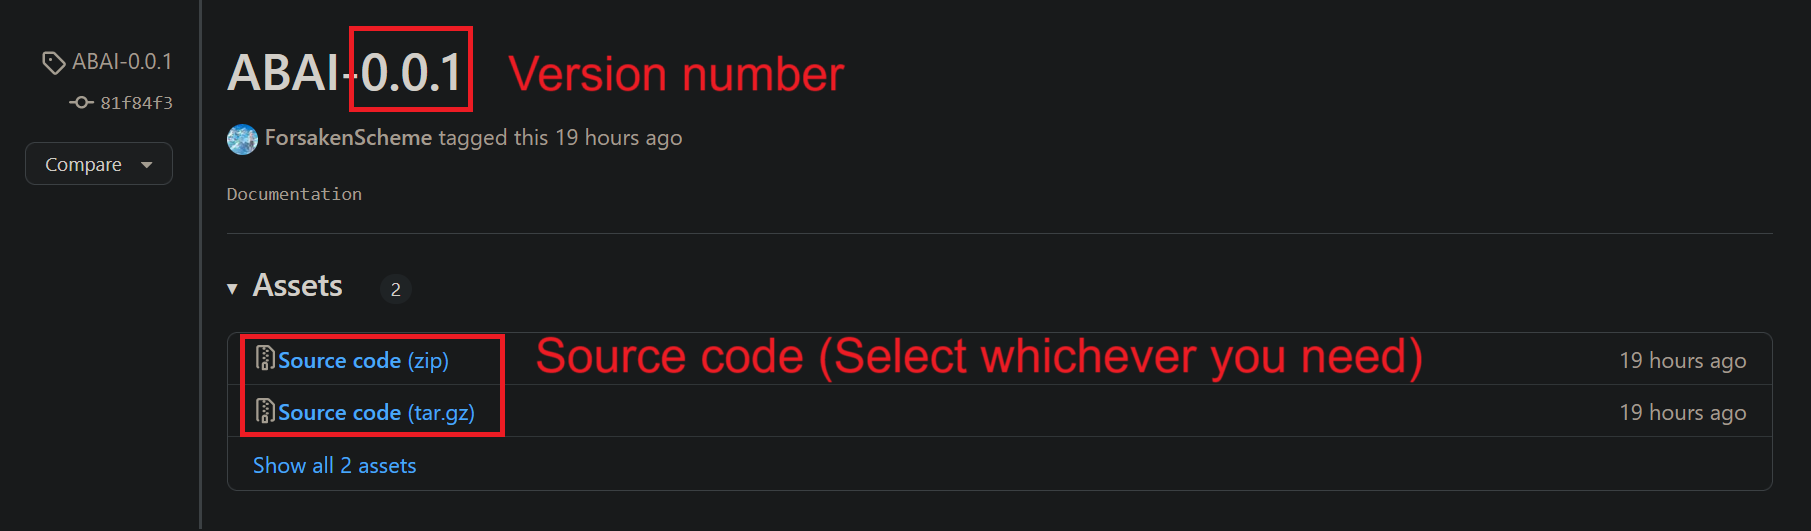
\includegraphics[width=17cm]{Images/Download/releases.png}
\end{center}
\subsection{Extract}
\label{subsec:Extract}
Once the download is complete, select your favourite extraction method (built-in OS feature or any additional file archiver software like \href{https://7-zip.org/}{7-Zip}), and extract the content of the compressed project folder into the installation folder at the location of your choice.
\begin{center}
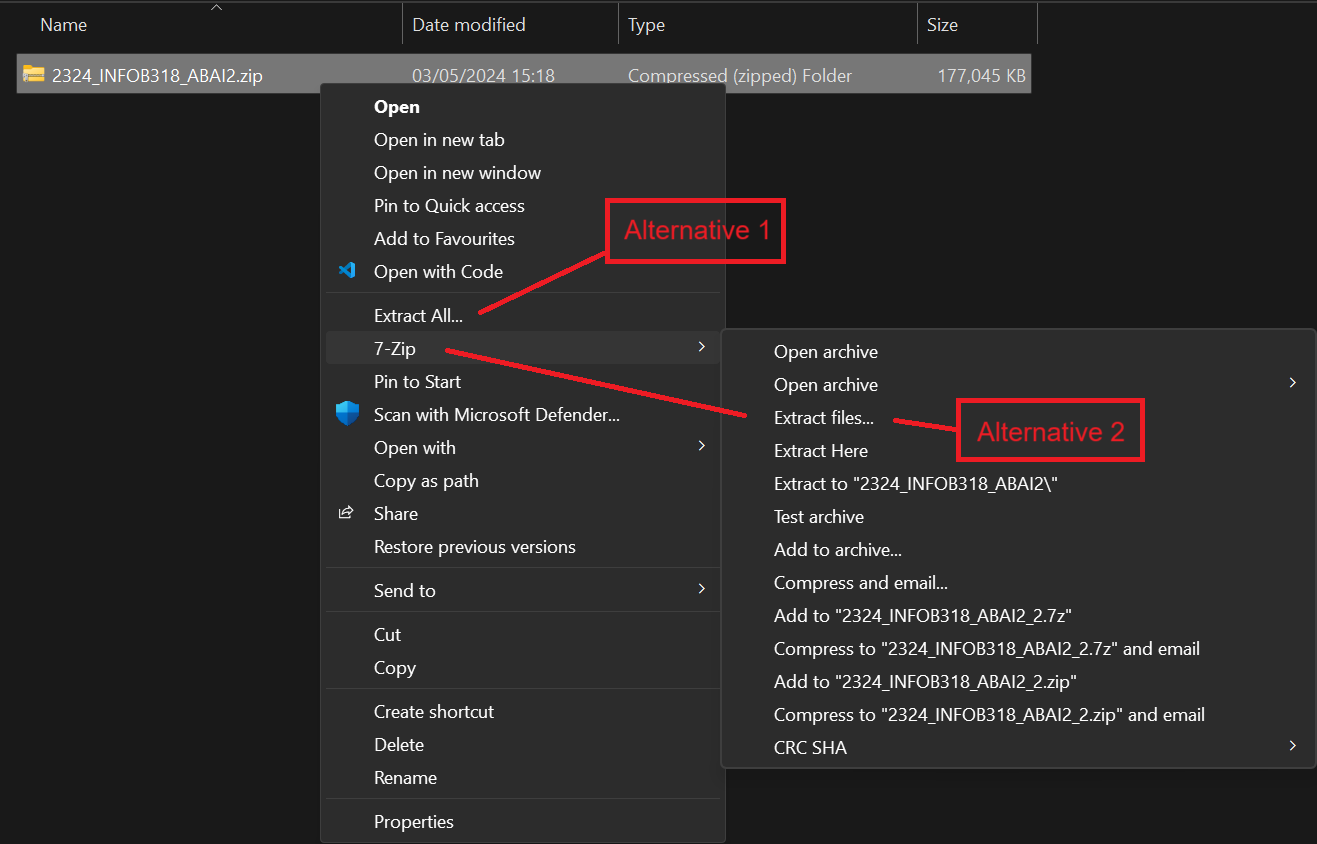
\includegraphics[width=17cm]{Images/Extract/Extraction.png}
\end{center}

After extraction, you should have the following folders: 
\begin{center}
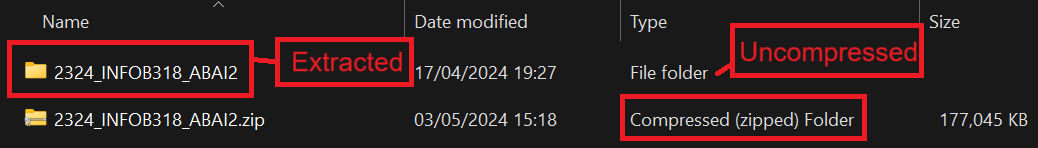
\includegraphics[width=17cm]{Images/Extract/after_extraction.png}
\end{center}

The uncompressed folder should contain the file structure shown as preview on the GitHub project page. The compressed folder can be safely deleted after having extracted and placed the \texttt{2324\_INFOB318\_ABAI2-[\texttt{version number}]} folder where you want to store it to run the program from.


\subsection{First steps}
\label{subsec:First steps}
After finishing the previous steps (\hyperref[subsec:Requirements]{2.1}, \hyperref[subsec:Download]{2.2}, \hyperref[subsec:Extract]{2.3} and \hyperref[subsec:First steps]{2.4}), you should now be able to start the tool. The steps to start ABAI may vary depending on what features and platform you plan to use. A walk-trough with steps for the local and web based application can be found at section \hyperref[subsubsec:Local application]{2.4.1 Local application} and \hyperref[subsubsec:Web application]{2.4.2 Web application}.

\subsubsection{Local application}
\label{subsubsec:Local application}
If you want to start the local application, you will have to use the standalone \textbf{python} GUI. For this, proceed as follows : 

\begin{itemize}
  \item Navigate to the \texttt{2324\_INFOB318\_ABAI2-[\texttt{version number}]} folder and, inside the folder, run the command:\begin{codebox}
    \texttt{pip install -r requirements.txt}.
  \end{codebox}
  \item Still inside the folder, run the command: 
  \begin{codebox}
    \texttt{python -O .\textbackslash code\textbackslash backend\textbackslash main.py}.
  \end{codebox}
  \item A window will open, this is the python GUI menu. 
\end{itemize}
\clearpage
\subsubsection{Web application}
\label{subsubsec:Web application}
If you want to start the web application, you are able to use the command-line terminal with Python or Docker (Docker Desktop GUI). 

\paragraph{\fontsize{14}{17}\selectfont Python}
\begin{itemize}
  \item First, open a terminal and navigate to the \texttt{2324\_INFOB318\_ABAI2-[\texttt{version number}]} folder.
  \item Inside the folder, run the command: 
  \begin{codebox}
    \large\texttt{pip install -r requirements.txt}.
  \end{codebox}
  \item Still inside the folder, run the command:
  \begin{codebox}
    \large\texttt{python -O .\textbackslash code\textbackslash django\_abai\textbackslash manage.py runserver 0.0.0.0:8000}.
  \end{codebox}
  \item Open your favorite browser and go to: \url{http://localhost:8000/}.
\end{itemize}
\paragraph{\fontsize{14}{17}\selectfont Docker}
\begin{itemize}
  \item First, open a terminal and navigate to the \texttt{2324\_INFOB318\_ABAI2-[\texttt{version number}]} folder.
  \item From the current working directory, run the command:
  \begin{codebox}
    \texttt{docker-compose -f docker/docker-compose.yml build}.
  \end{codebox}
  \item Then,  still from the \texttt{2324\_INFOB318\_ABAI2-[\texttt{version number}]} current working directory, run the command:
  \begin{codebox}
    \texttt{docker-compose -f docker/docker-compose.yml up abai-website}
  \end{codebox}
  \textbf{or} \\
  On the Docker Desktop GUI chose the abai-web image and start the container with a name of your choice and specify the port 8000.
  \item Open your favourite browser and go to: \\
  \url{http://172.28.112.1:8000/} (accessible from any device in the local network) \\
  \textbf{or} \\
  \url{http://localhost:8000/} (accessible from local host device only).
\end{itemize}



\clearpage
\section{Usage}
ABAI can be broken down into two smaller programs. You will be able to use the \textbf{local application} if you want to customize the data, the models and their feature extraction processes. The \textbf{web based application} is a simplified tool that uses pre-trained models to perform the authorship attribution task based on the model you select. 

\subsection{Local application}
The GUI for the local application consists of a main application window and is then divided into multiple sub-windows for each menu option. If you close the main window or any sub-window, their child windows will also be closed. 
\begin{center}
    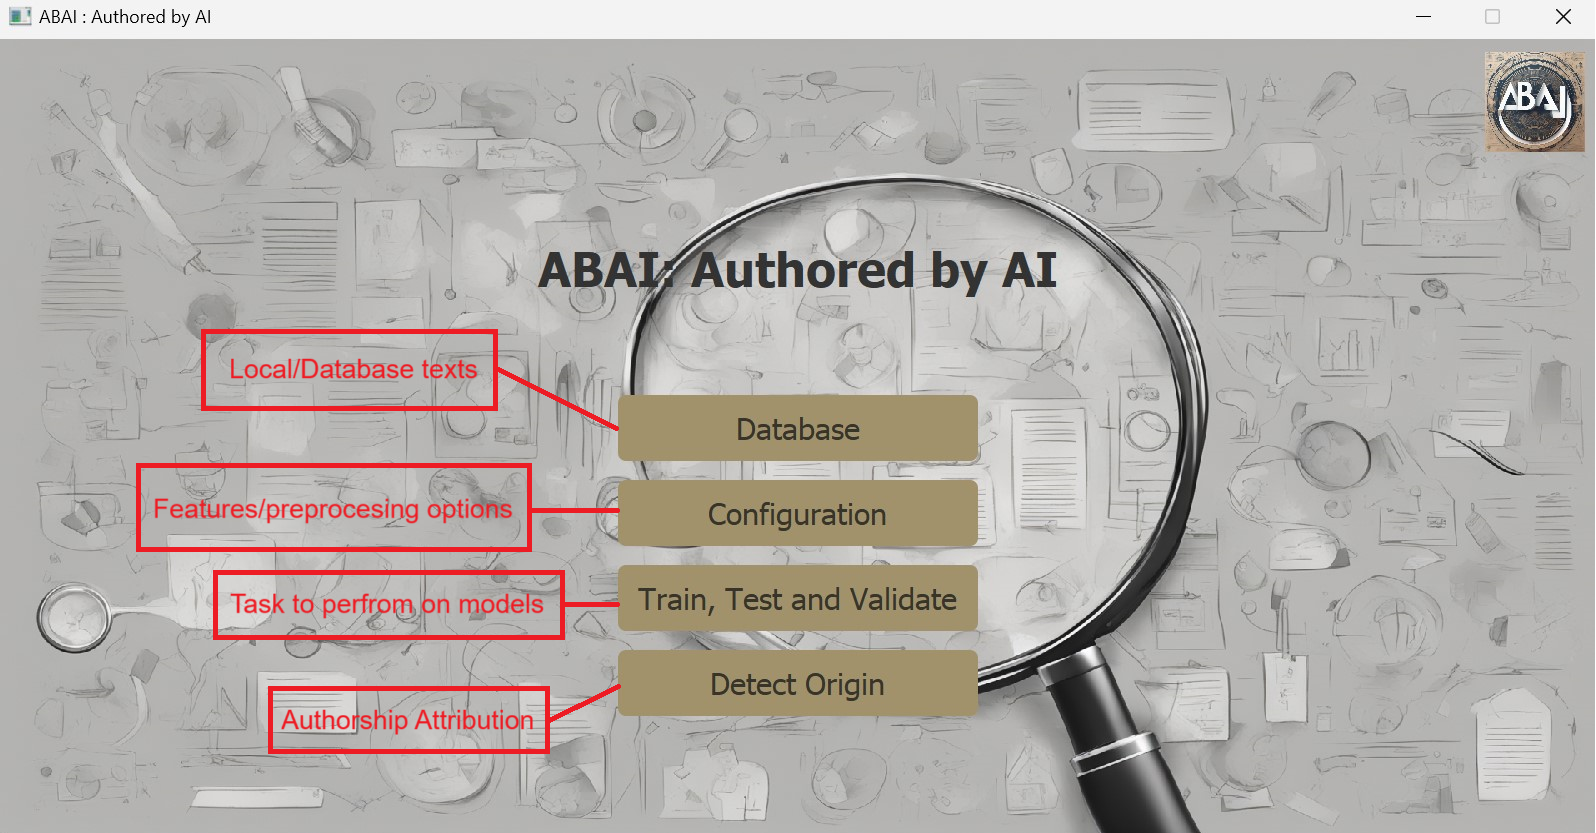
\includegraphics[width=17cm]{Images/Usage/Local/MainWindow.png}
\end{center}
Now, let's break down the menu and it's options into smaller parts further explained in the following sections.
\clearpage
\subsubsection{Database}
\label{subsubsec:database}
In the database sub-window, you will be able to modify everything related to the databases and local files ABAI will draw from during the training of it's models. It's possible to add/remove directly to/from the \texttt{SQLite} database as well as storing local \texttt{.TXT} files. 
\begin{center}
    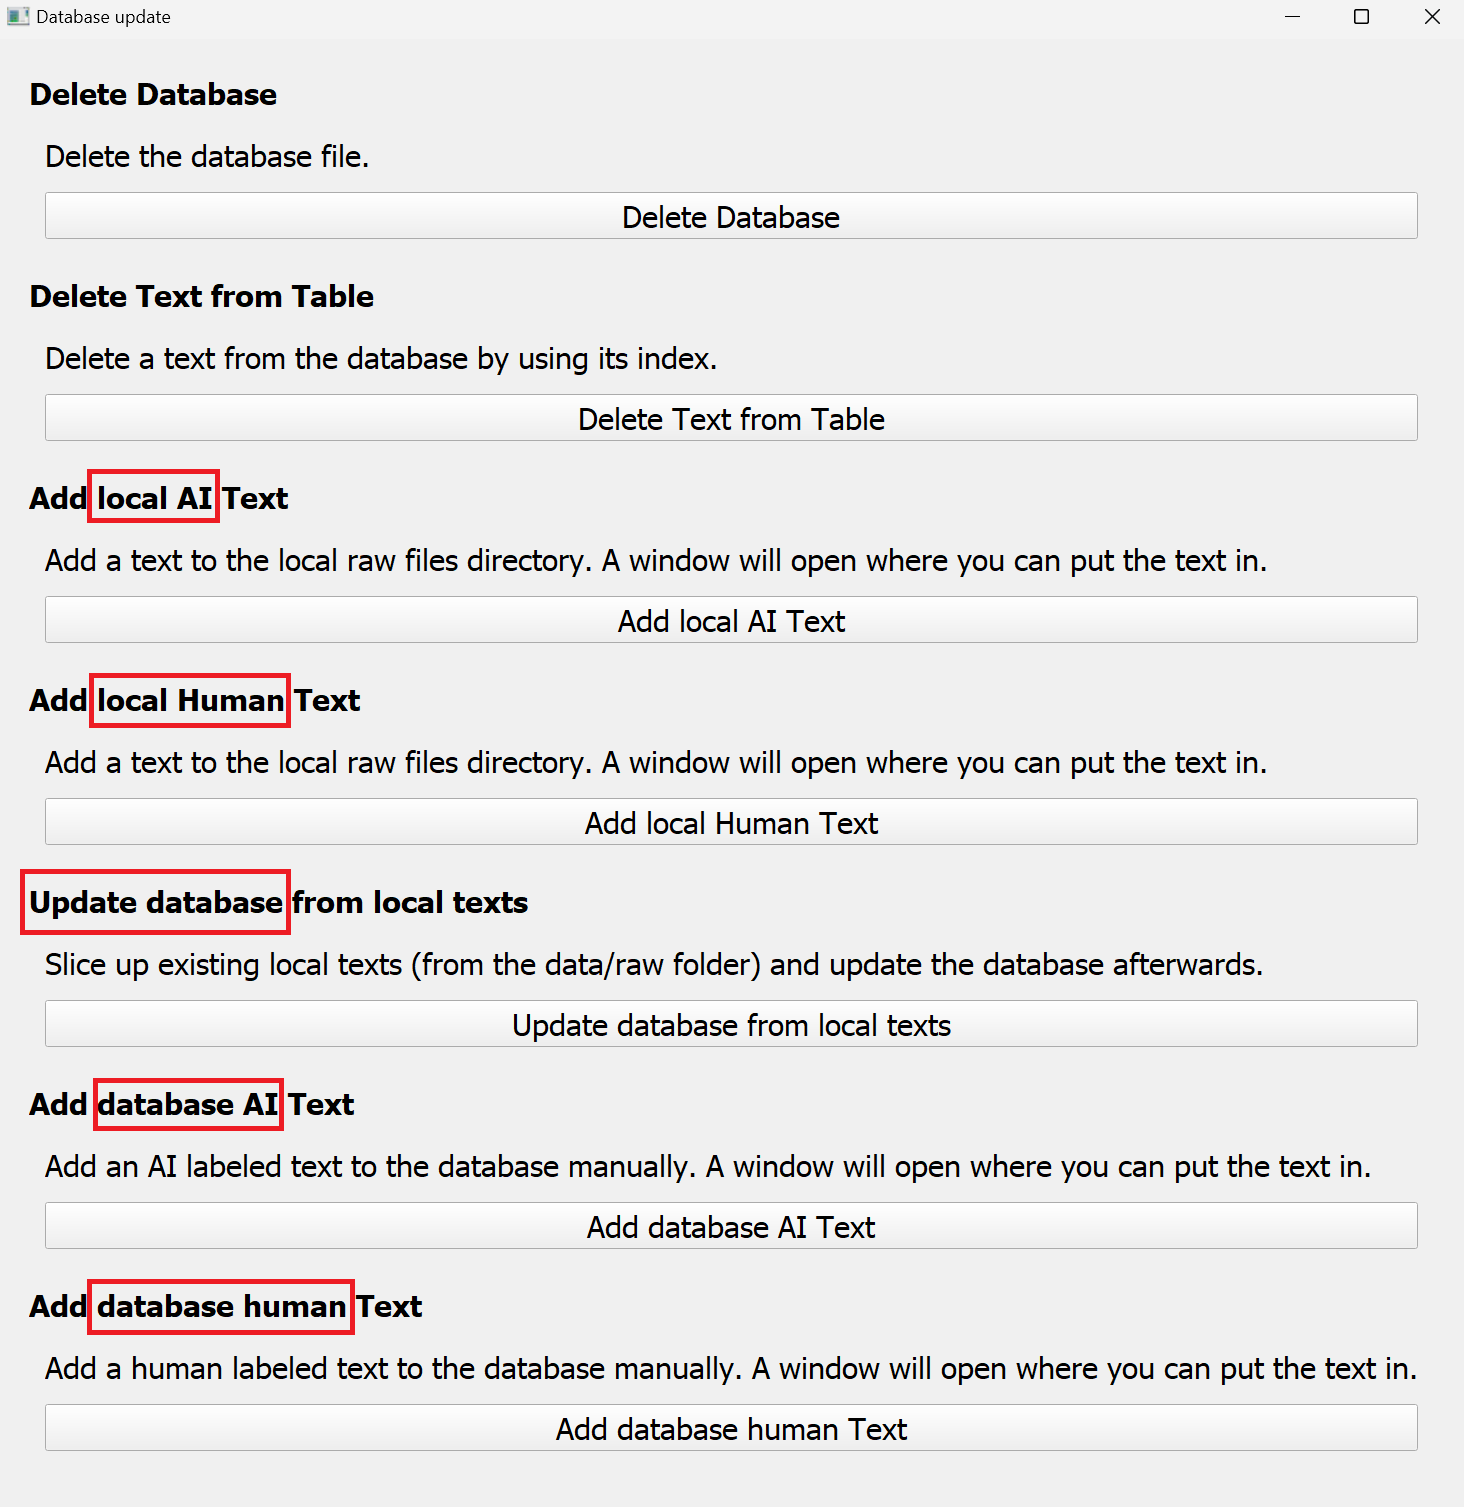
\includegraphics[width=17cm]{Images/Usage/Local/DatabaseWindow.png}
\end{center}
\clearpage
\subsubsection{Configuration}
In the configuration sub-window, you will be able to set options for different methods of feature extraction, cross-validation and random state used during processing tasks. 
\begin{center}
    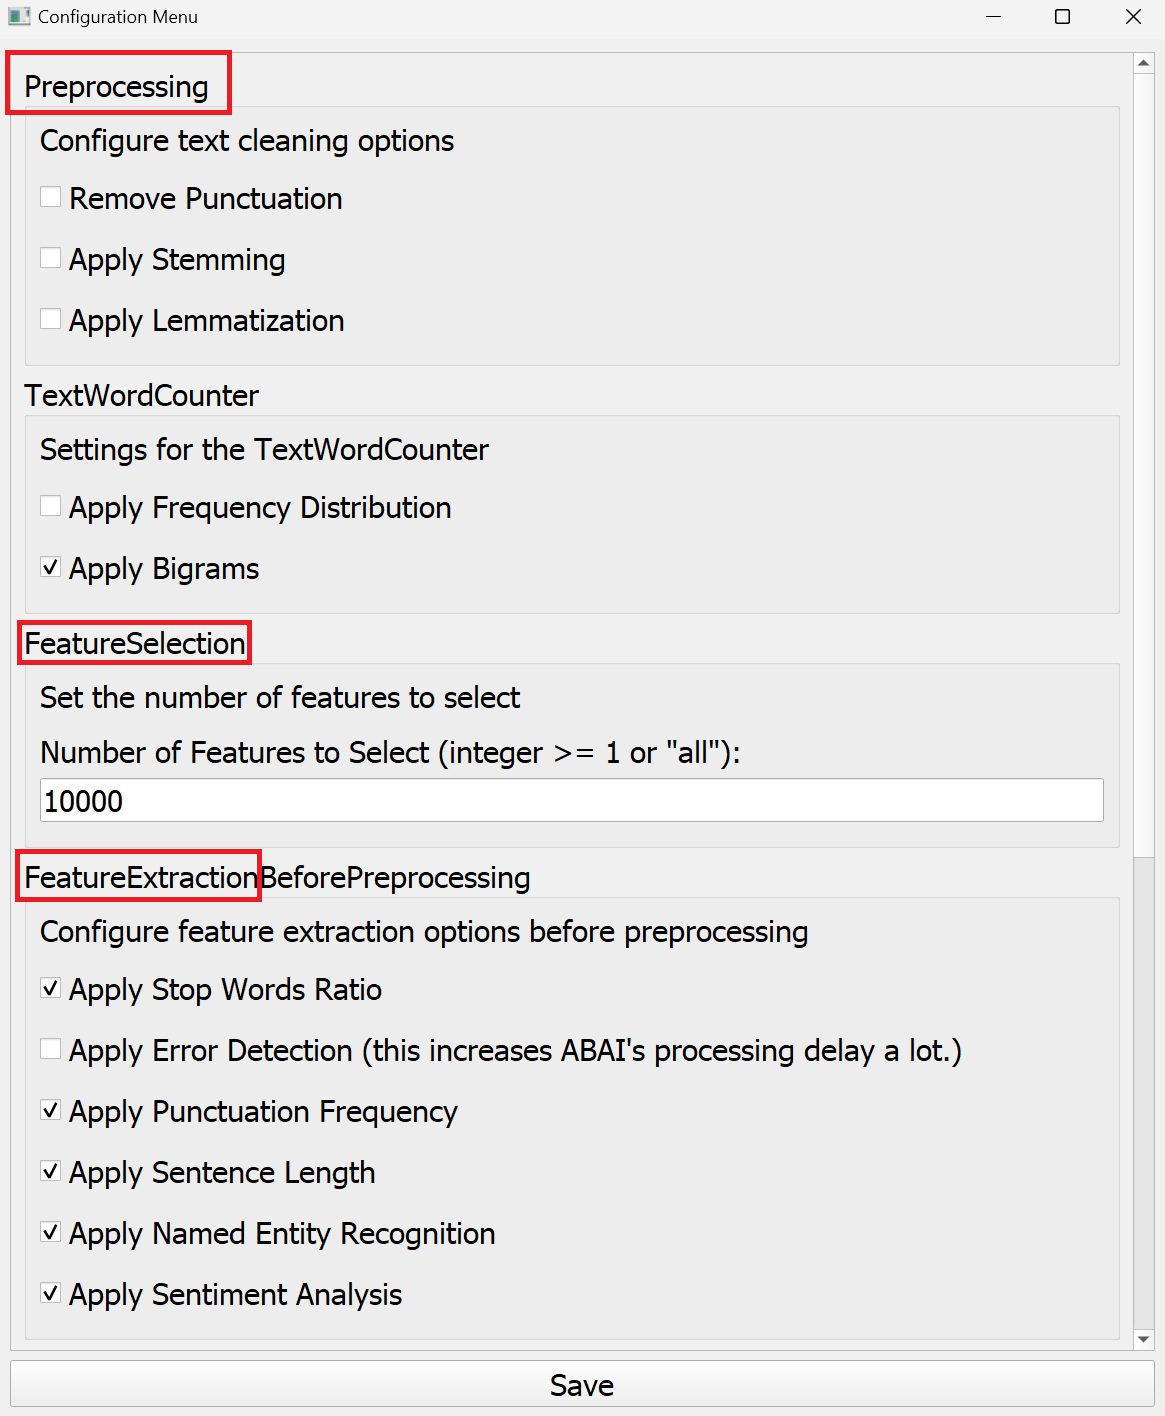
\includegraphics[width=17cm]{Images/Usage/Local/ConfigurationWindow.png}
\end{center}
\clearpage
\paragraph{\fontsize{14}{17}\selectfont A brief explanation}
\label{subsubsec:config-brief-explain}
\begin{itemize}
    \item \textbf{Preprocessing}\\\\
    Configure the text cleaning options. These options include removing punctuation, applying stemming, and lemmatization.\\
    
    \item \textbf{TextWordCounter}\\\\
    Choose between frequency distribution or tf-idf calculation, as well as whether to include bigrams in addition to unigrams.\\
    
    \item \textbf{FeatureSelection}\\\\
    Specify the number of features to select for Kbest feature selection using the chi2 function. This setting allows you to control the dimensionality of your features.\\
    
    \item \textbf{FeatureExtractionBeforePreprocessing}\\\\
    This segment includes several feature extraction options that will be performed before preprocessing. These include applying stop words ratio, error detection for grammar and misspells (which may prolong the processing time because of API calls), punctuation frequency, average sentence length, named entity recognition, and sentiment analysis.\\
    
    \item \textbf{FeatureExtractionAfterPreprocessing}\\\\
    Apply additional feature extraction methods that will be performed after preprocessing. These include text word counting, average word length, and vocabulary size.\\
    
    \item \textbf{CrossValidation}\\\\
    Set the number of folds for cross-validation.\\
\end{itemize}

\subsubsection{Train, Test, and Validate}
\label{subsubsec:train-test-validate}
In the train, test and validate sub-window you will be able to select the models you want to use (multiple simultaneous selections are allowed) and which task you want to perform for them. After the task has finished, a new window will open with the result.
\begin{center}
    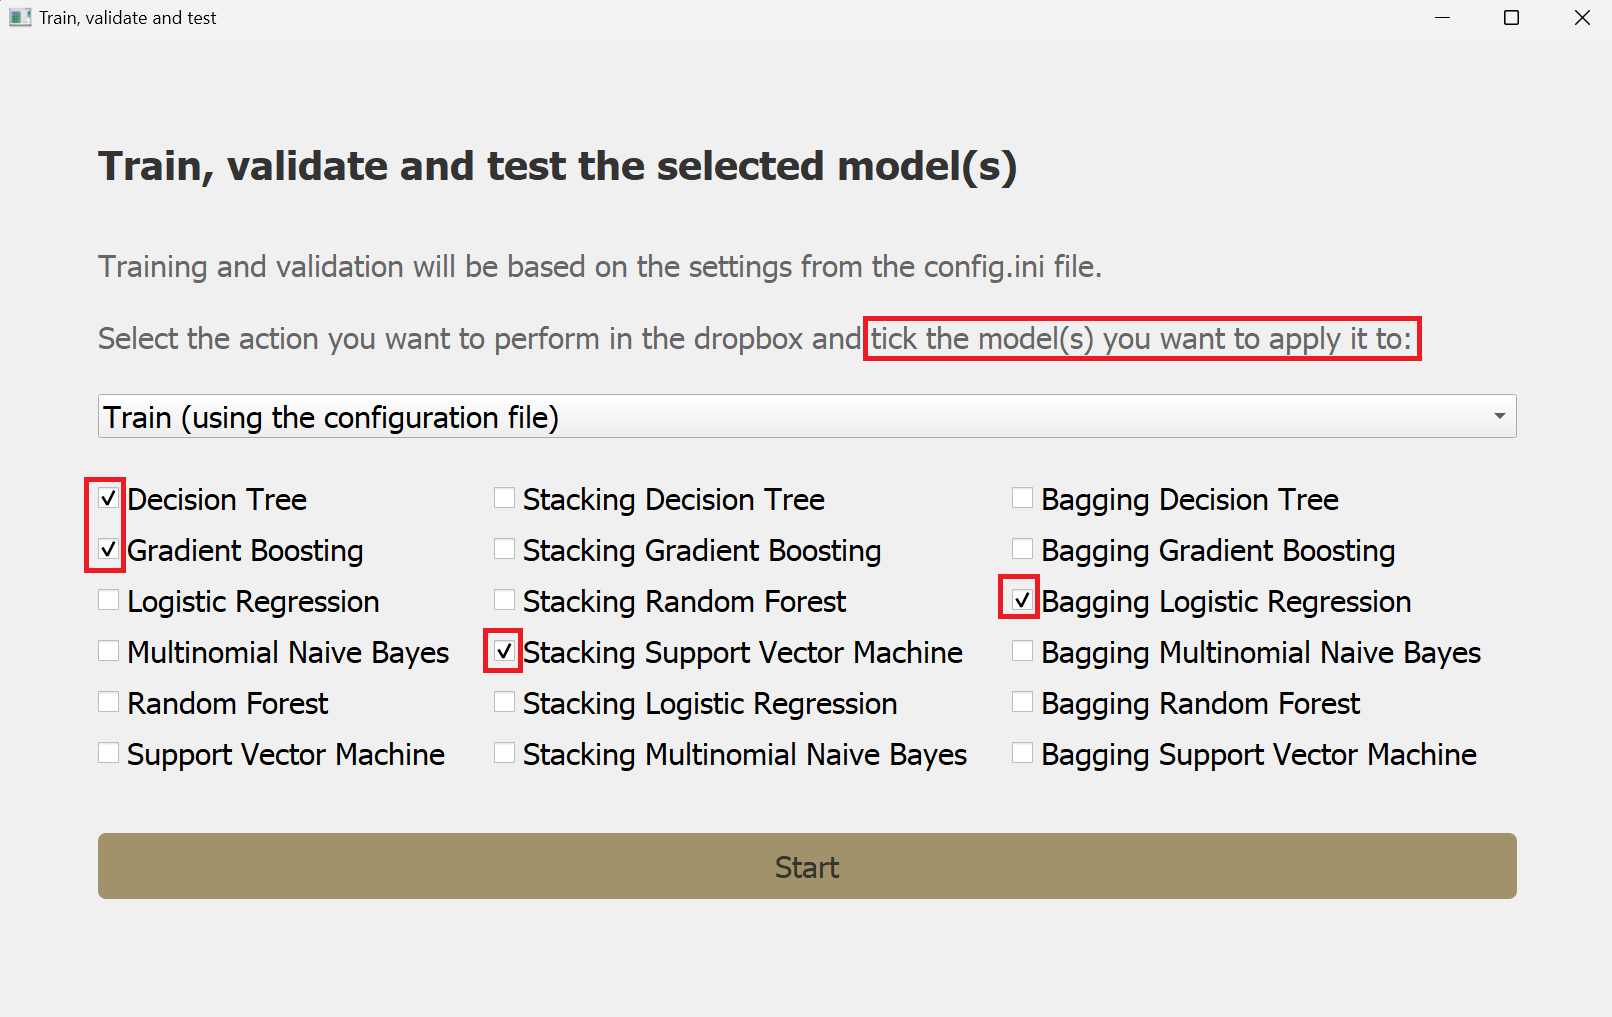
\includegraphics[width=16cm]{Images/Usage/Local/Train-Test-Validate-Window1.png}
\end{center}
\begin{center}
    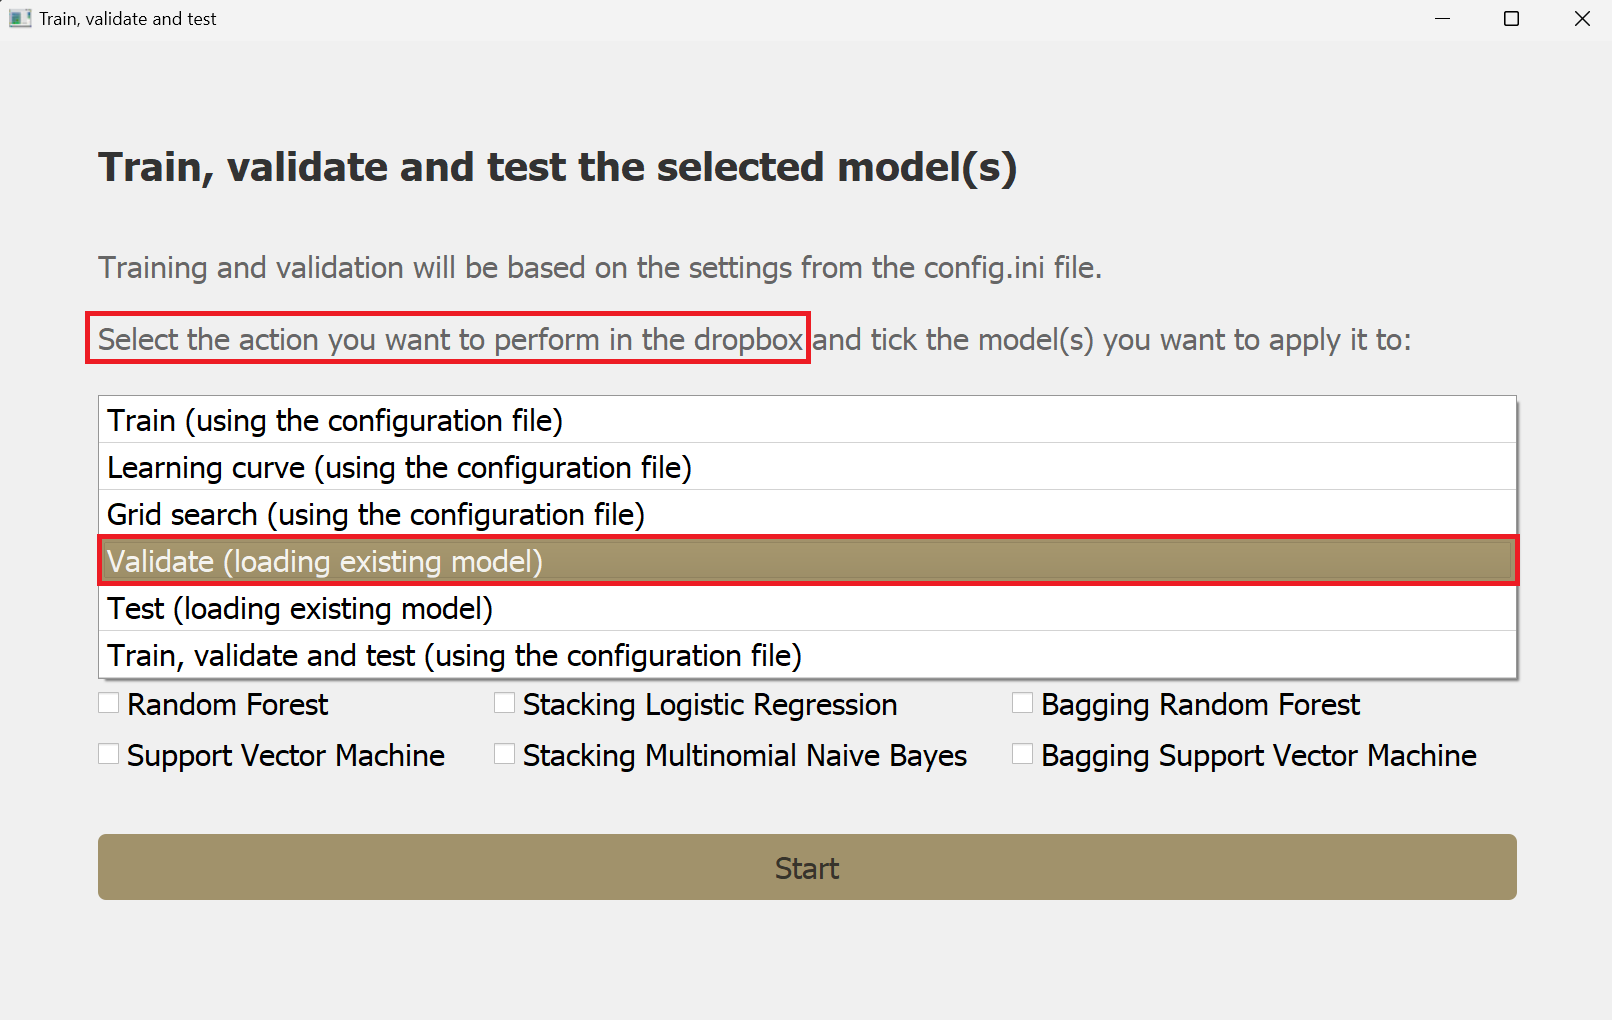
\includegraphics[width=16cm]{Images/Usage/Local/Train-Test-Validate-Window2.png}
\end{center}
\subsubsection{Detect Origin}
In the detect origin sub-window you will be able to select the model you want to use to perform the authorship detection task with. Copy and paste the text you want to analyze into the corresponding text box. Then press the \texttt{Detect Origin} button and wait for the task to finish. A new window will open with the result.
\begin{center}
    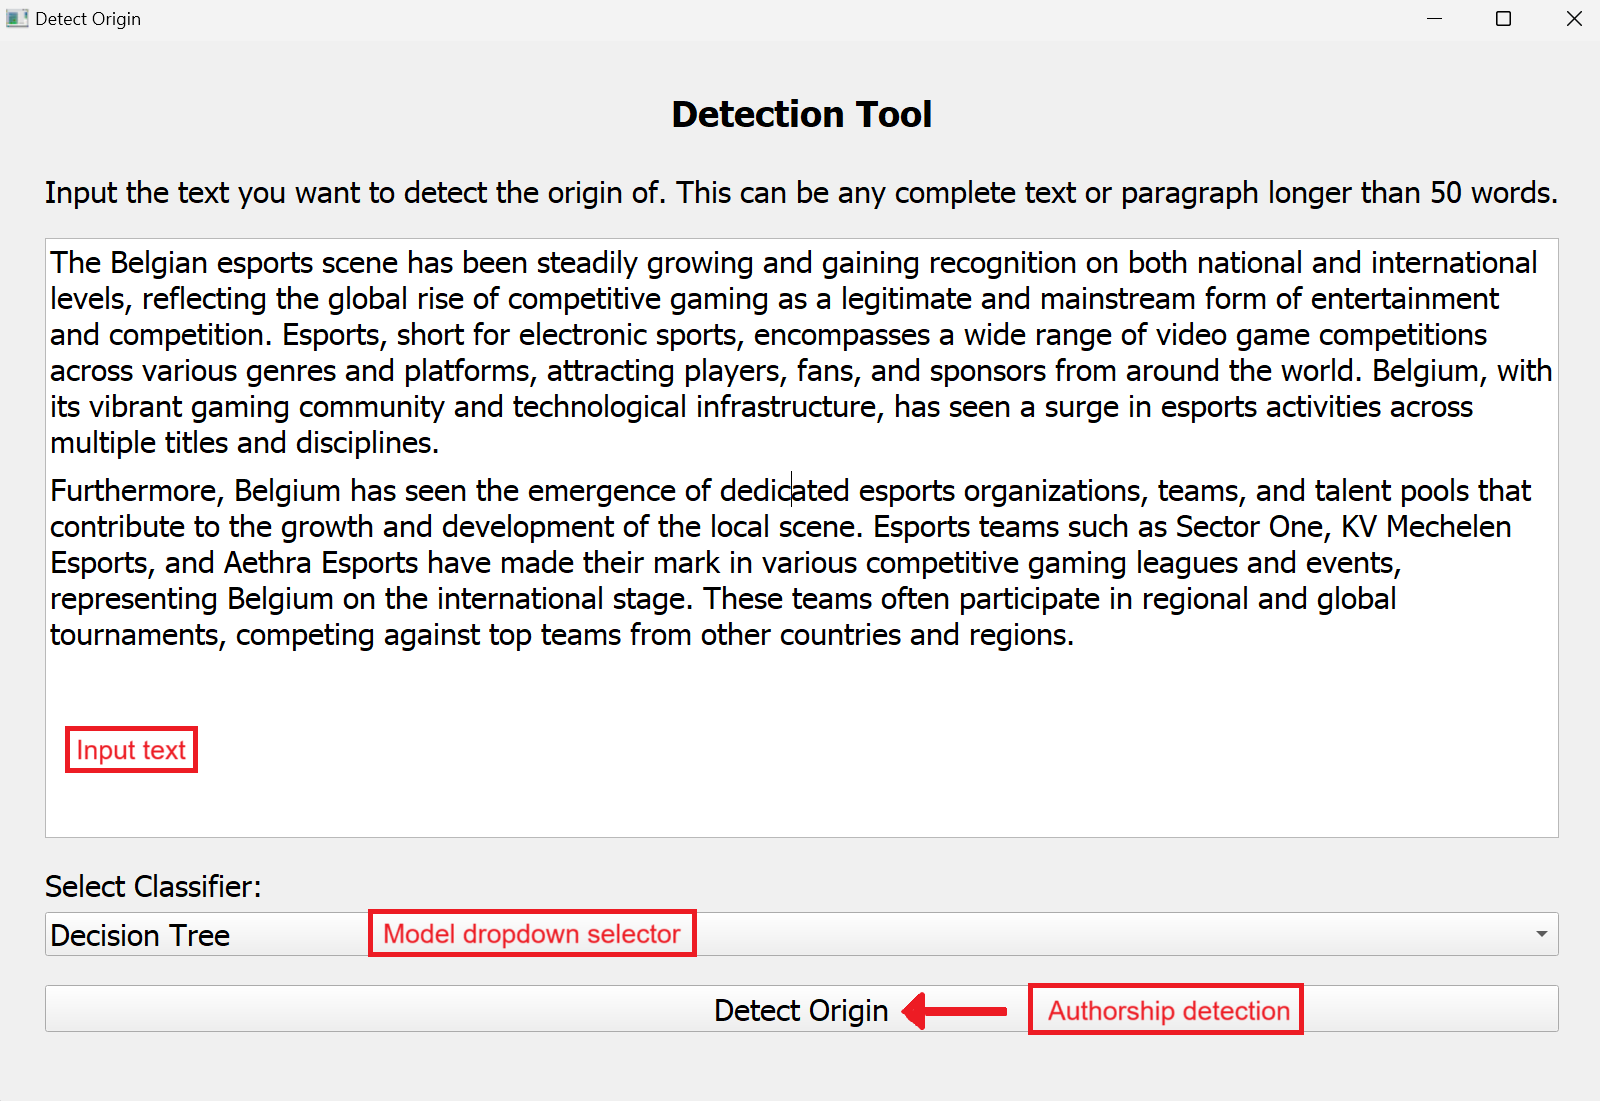
\includegraphics[width=17cm]{Images/Usage/Local/Detect-Origin-Window.png}
\end{center}
\clearpage
\subsection{Web based application}
The web application has a simplified interface. It contains text guidance on how to use the authorship detection feature, a text box to input the text to be analyzed and a button to start the process.
\begin{center}
    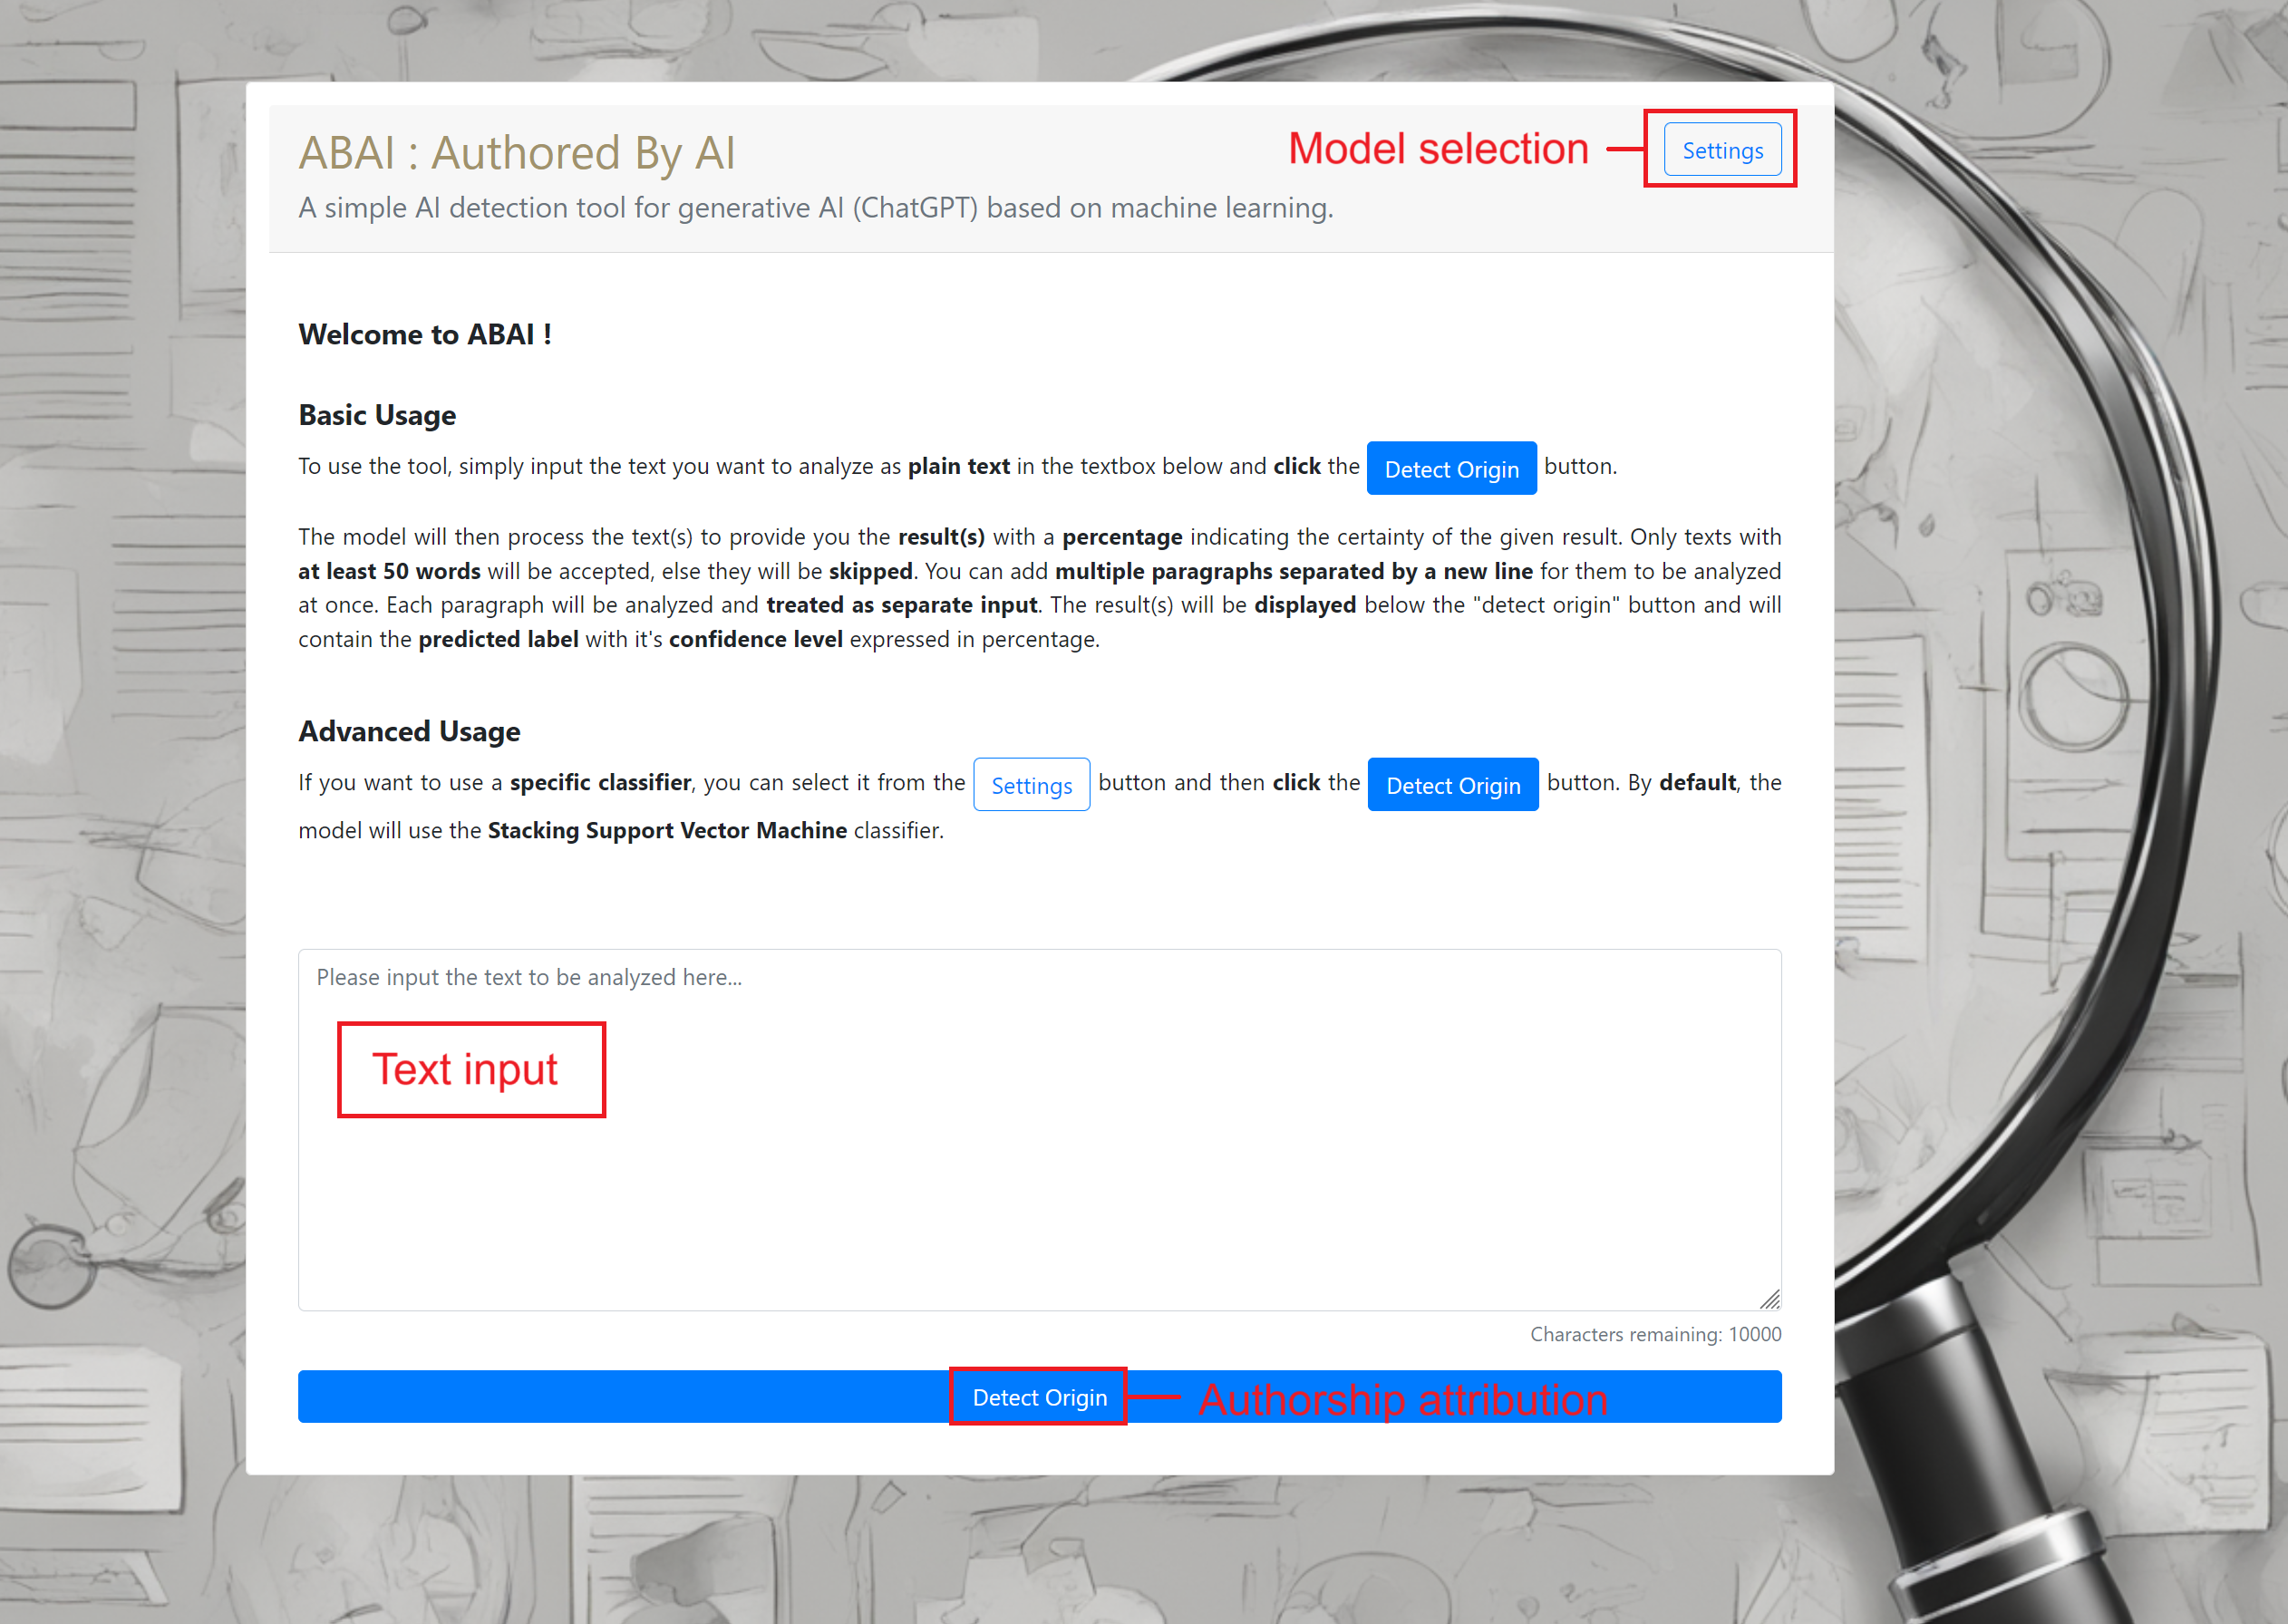
\includegraphics[width=17cm]{Images/Usage/Web/Web-application.png}
\end{center}
For a comparison between the different pre-trained models, the advanced usage let's you select a different model than the default one (Stacking Support Vector Machine). You do this by pressing the settings button situated in the top-right corner of the interface.
\begin{center}
    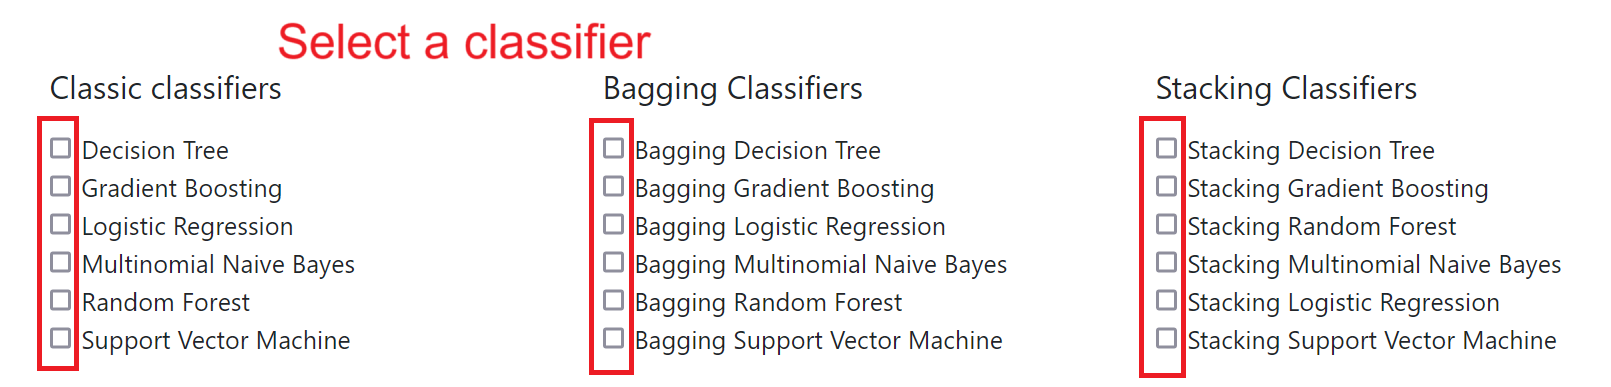
\includegraphics[width=17cm]{Images/Usage/Web/Web-settings.png}
\end{center}
When ready, press the \texttt{detect origin} button and wait for the results to be displayed bellow the \texttt{Detect Origin button}.
\begin{center}
    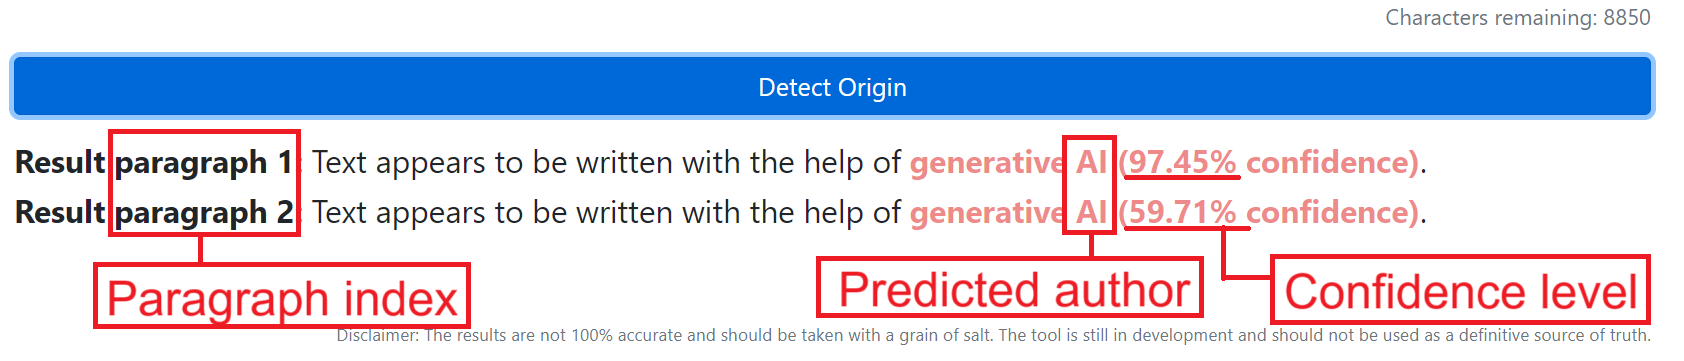
\includegraphics[width=17cm]{Images/Usage/Web/Web-results.png}
\end{center}

\subsection{How to guides}
\subsubsection{How to use the web/local application to detect the author of a given text?}
\begin{enumerate}
    \item Open the \hyperref[subsubsec:Web application]{web-based} version of the application or launch the \hyperref[subsubsec:Local application]{local} application using the appropriate method from the \hyperref[subsec:First steps]{installation} steps.
    
    \item Once the application started, locate the \textbf{input box} (navigate to the \texttt{Detect Origin} window for the local application) where you can paste the text to be analyzed. Copy the text you want to analyze and paste it there. Ensure that the text does not exceed the maximum \textbf{10 000 character limit} for the web application. 
    \begin{center}
        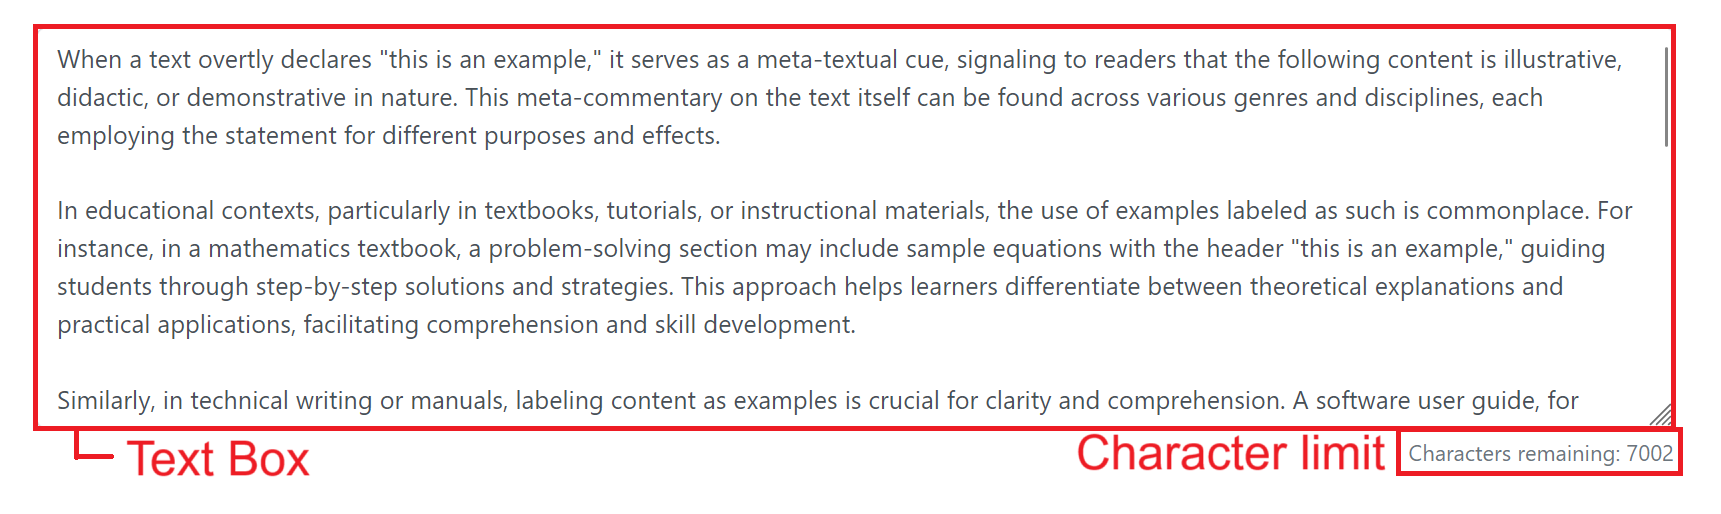
\includegraphics[width=17cm]{Images/Usage/Demo/Paste-limit.png}
    \end{center}
    \item After pasting the text, look for the \texttt{Detect Origin} button and click it to initiate the analysis process.
    \begin{center}
        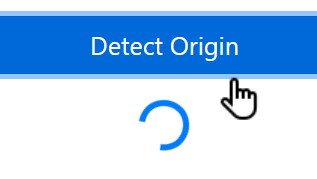
\includegraphics[width=4cm]{Images/Usage/Demo/Detect-load.png}
    \end{center}
    \item Wait for the analysis to complete. Depending on the complexity of the text and the processing steps, this may take a few moments.
    \item Once the analysis is finished, review the results displayed by the application. The results will indicate whether the text is likely to be authored by a human or generated by an AI model with a certain level of confidence. The result will also indicate if a paragraph doesn't meet a requirement like word length.
\begin{center}
    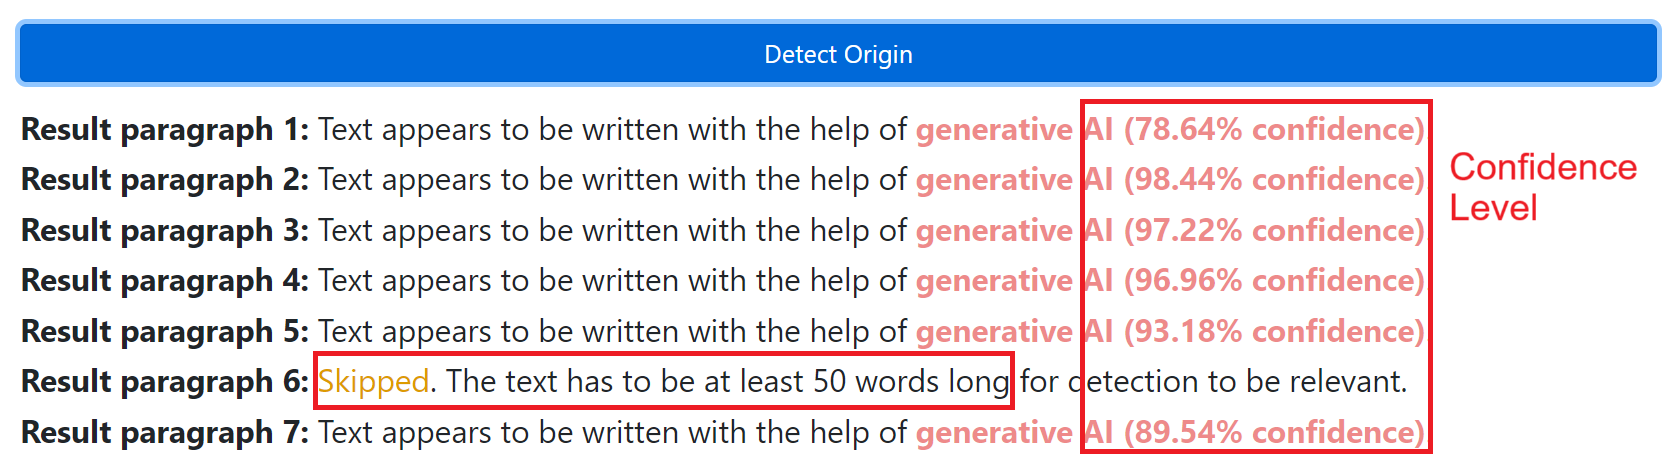
\includegraphics[width=16cm]{Images/Usage/Demo/Results.png}
\end{center}
\end{enumerate}

\subsubsection{How to use the local application to add local texts to the dataset?}
\begin{enumerate}
    \item Open the \hyperref[subsubsec:Web application]{web-based} version of the application or launch the \hyperref[subsubsec:Local application]{local} application using the appropriate method from the \hyperref[subsec:First steps]{installation} steps.
    \item Navigate from the main menu to the \hyperref[subsubsec:database]{Database} sub-window.
    \begin{center}
        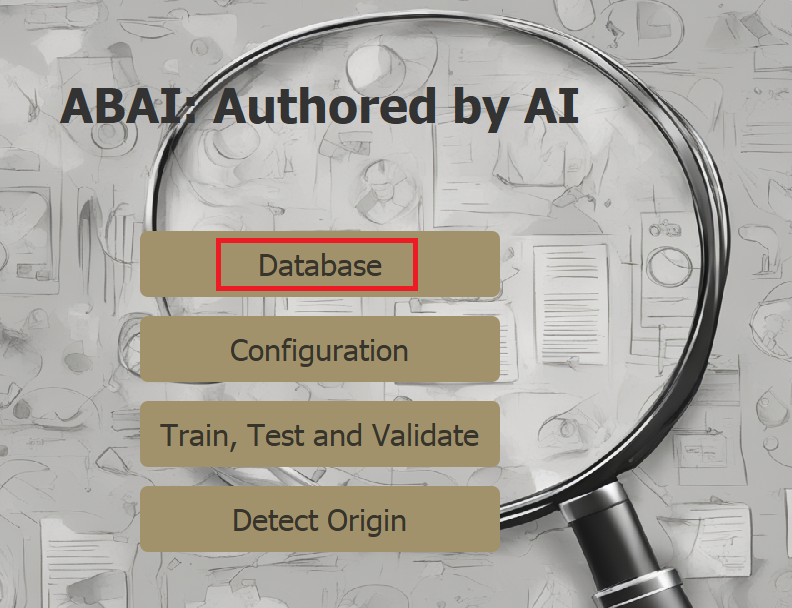
\includegraphics[width=16cm]{Images/Usage/Demo/navigate-database.png}
    \end{center}
    \item On the database sub-window select the button to add a text to the local texts with the corresponding label (human or AI).
    \begin{center}
        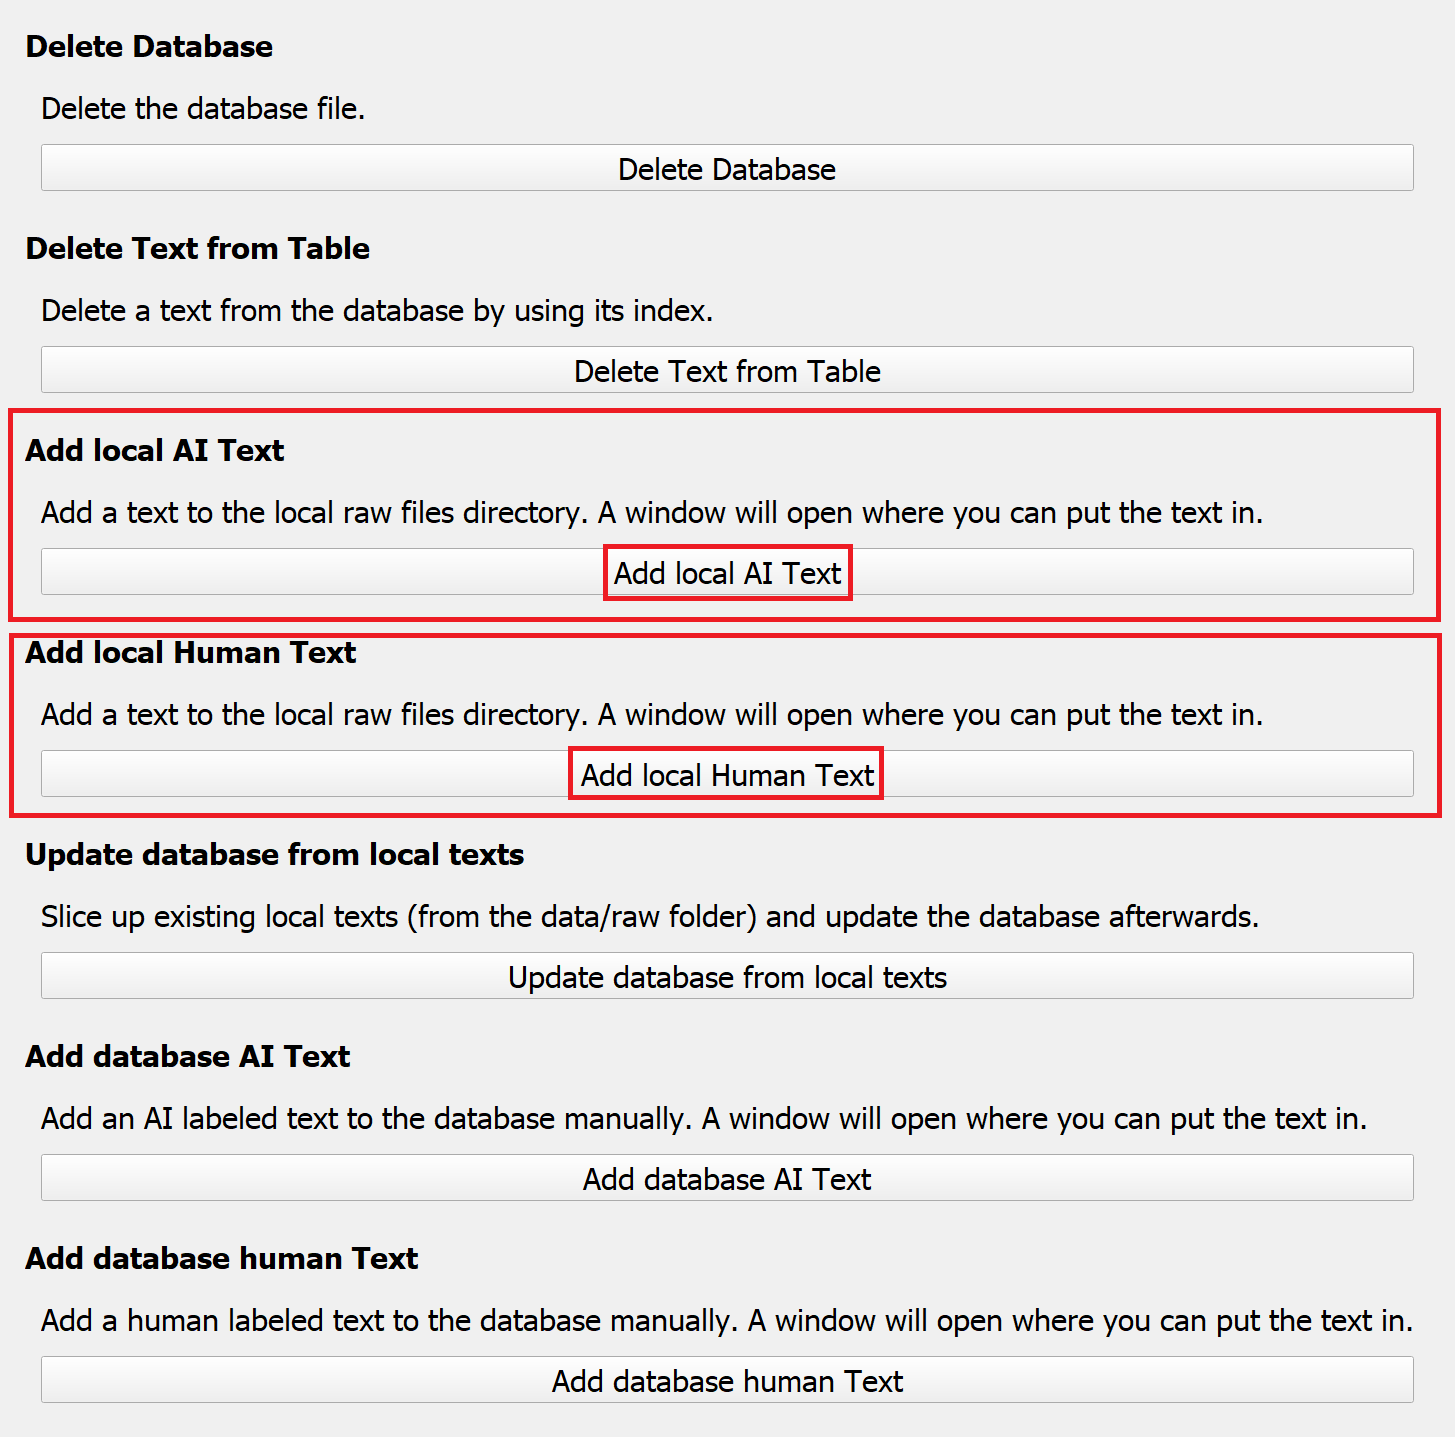
\includegraphics[width=14cm]{Images/Usage/Demo/Add-local.png}
    \end{center}
    \item Paste the text into the text box and click the \textbf{\texttt{OK}} button to save.
    \begin{center}
        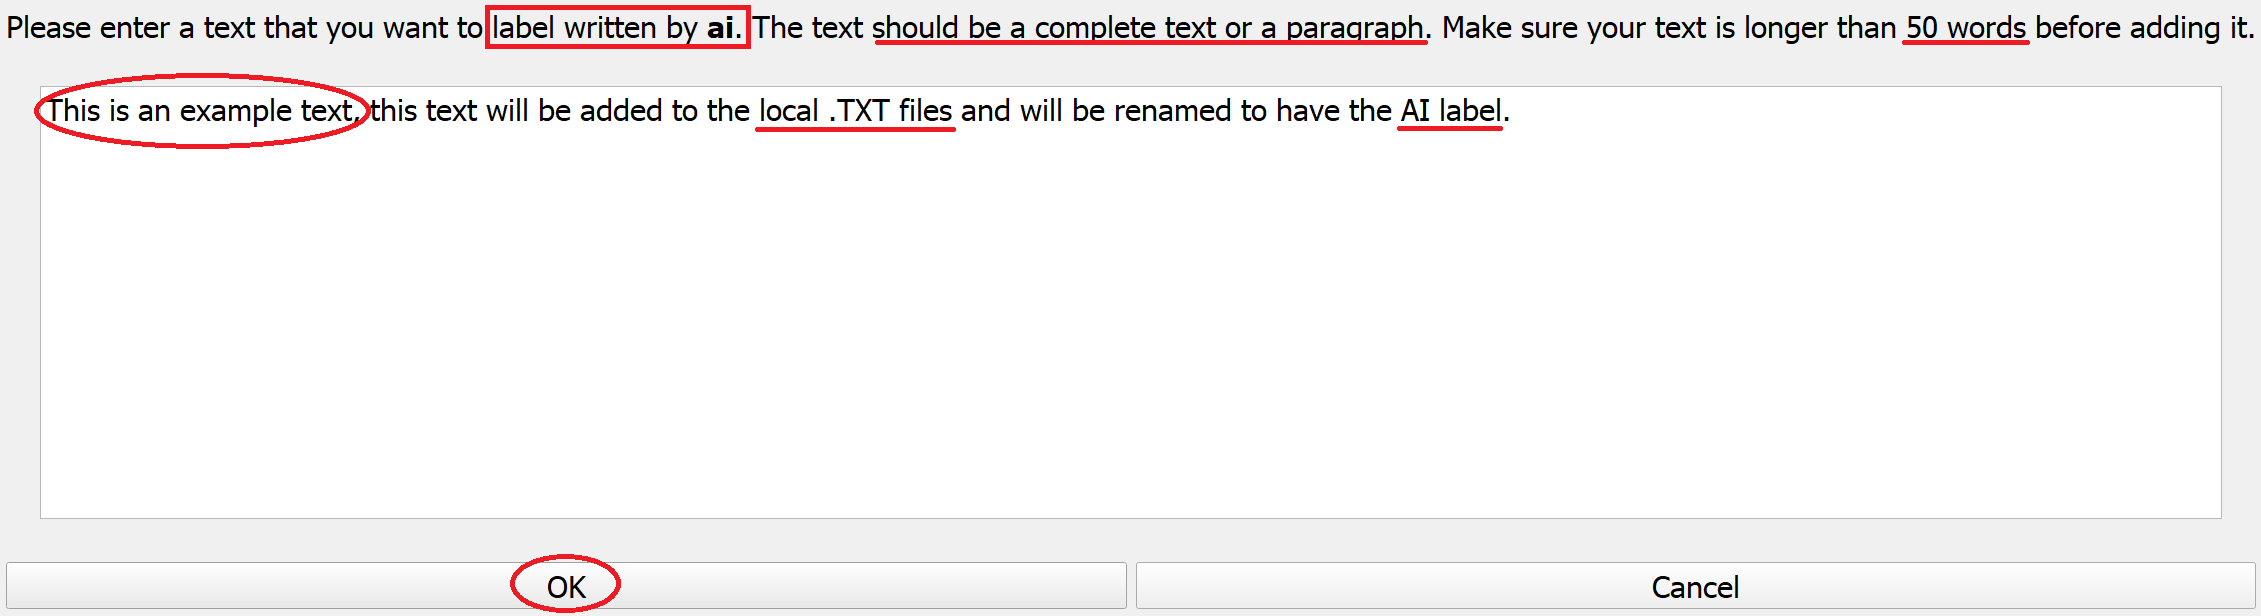
\includegraphics[width=16.5cm]{Images/Usage/Demo/Add-AI.png}
    \end{center}
    \clearpage
    \item Navigate back to the \hyperref[subsubsec:database]{Database} sub-window and click on the \texttt{Update database from local texts} button to include the freshly added local texts in the database.
    \begin{center}
        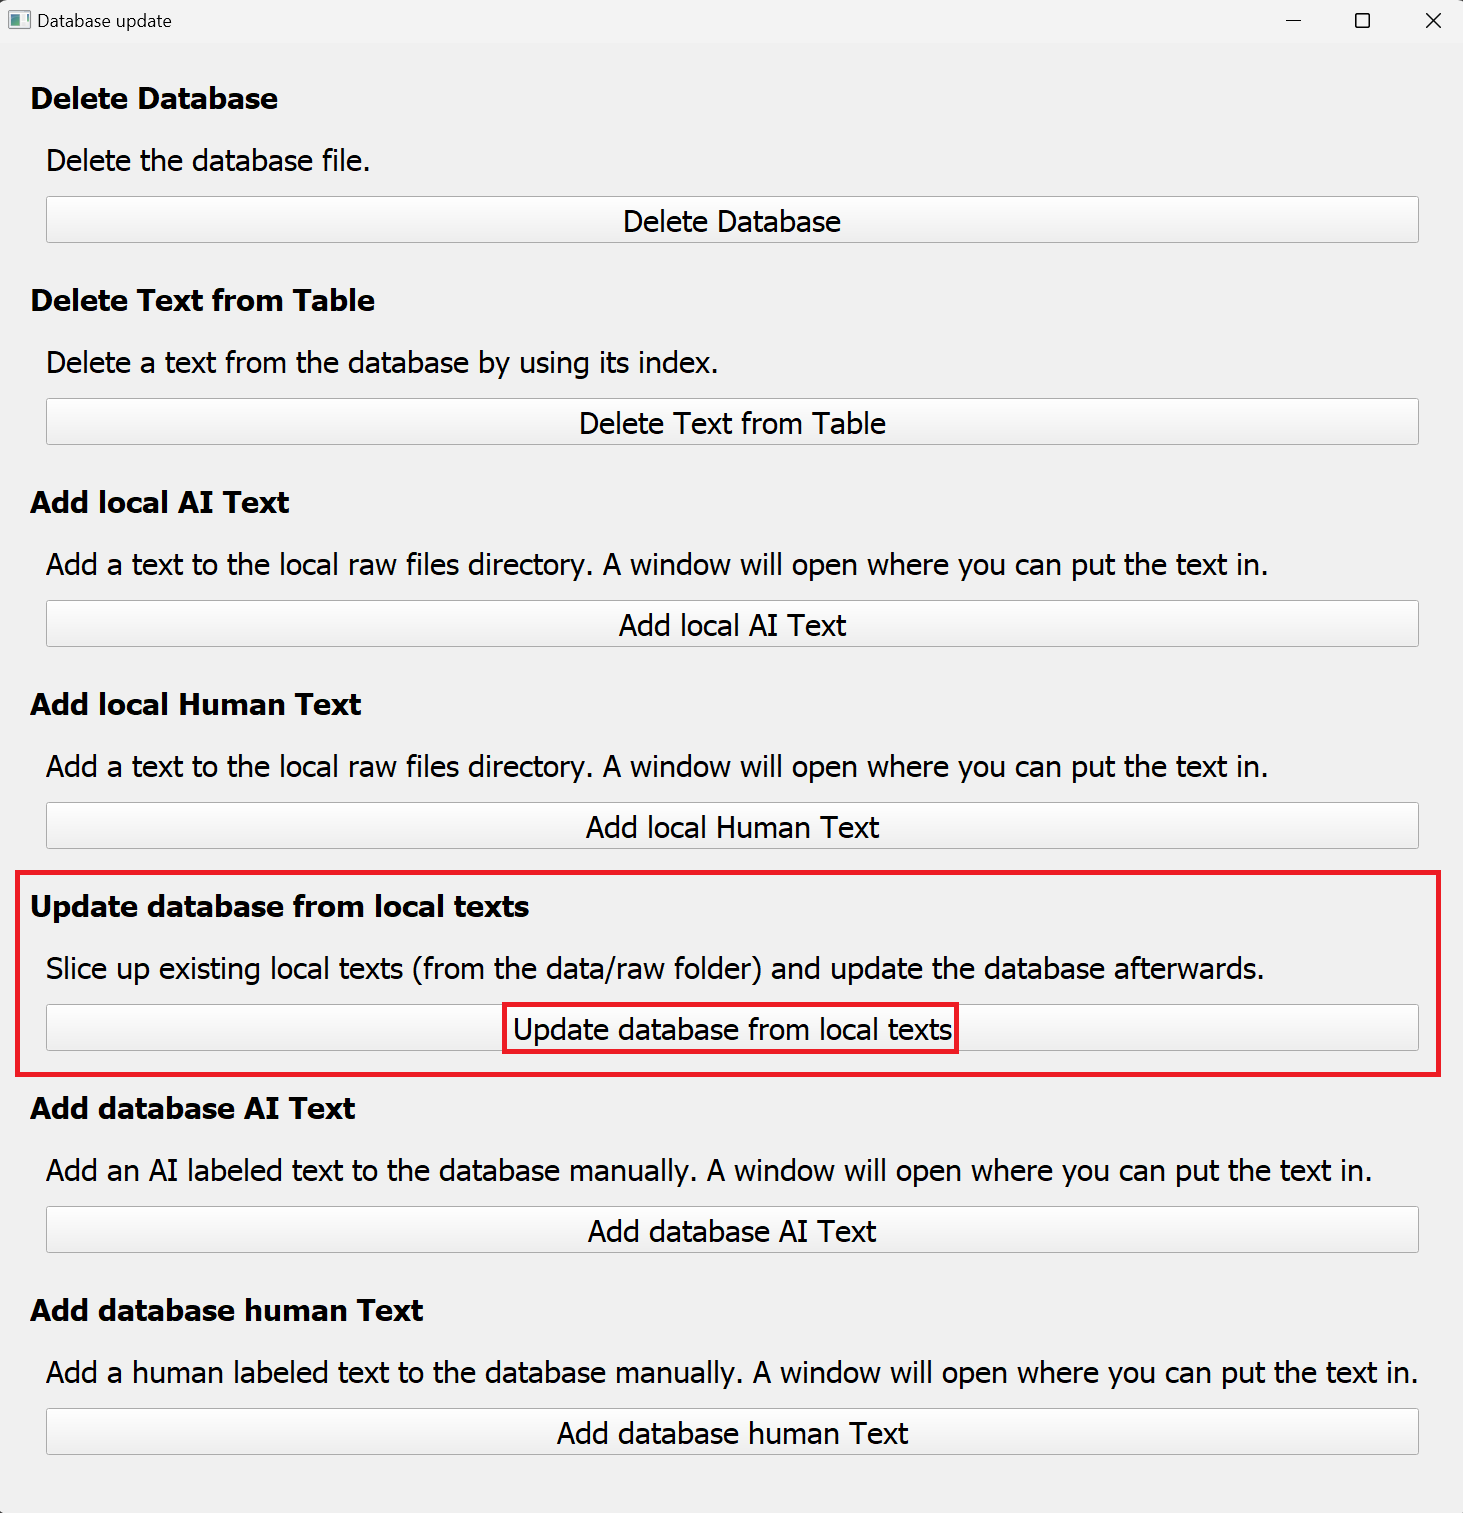
\includegraphics[width=16.5cm]{Images/Usage/Demo/Update-database.png}
    \end{center}
\end{enumerate}
\clearpage
\subsubsection{How to use the local application to delete texts from the dataset?}
\begin{enumerate}
    \item Open the \hyperref[subsubsec:Web application]{web-based} version of the application or launch the \hyperref[subsubsec:Local application]{local} application using the appropriate method from the \hyperref[subsec:First steps]{installation} steps.
    \item Navigate from the main menu to the \hyperref[subsubsec:database]{Database} sub-window.
    \begin{center}
        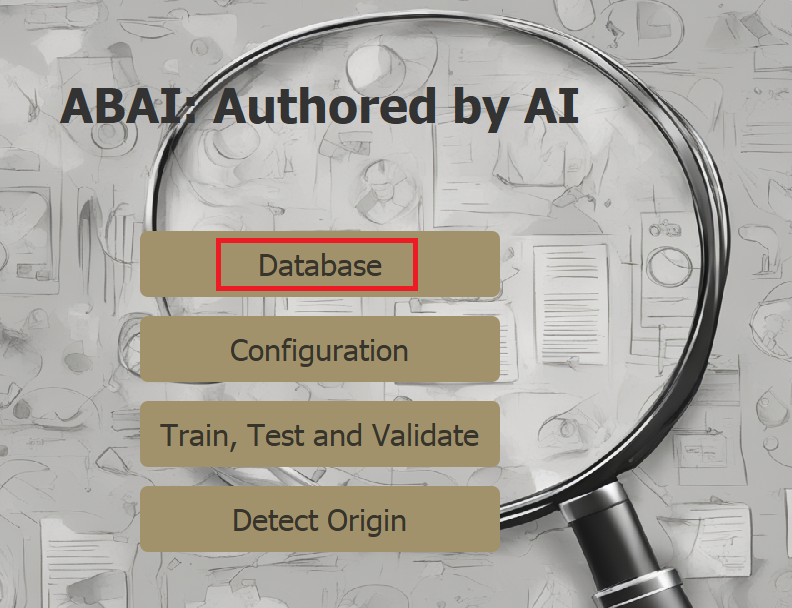
\includegraphics[width=11cm]{Images/Usage/Demo/navigate-database.png}
    \end{center}
    \item On the database sub-window select the button \texttt{Delete Text from Table}.
    \begin{center}
        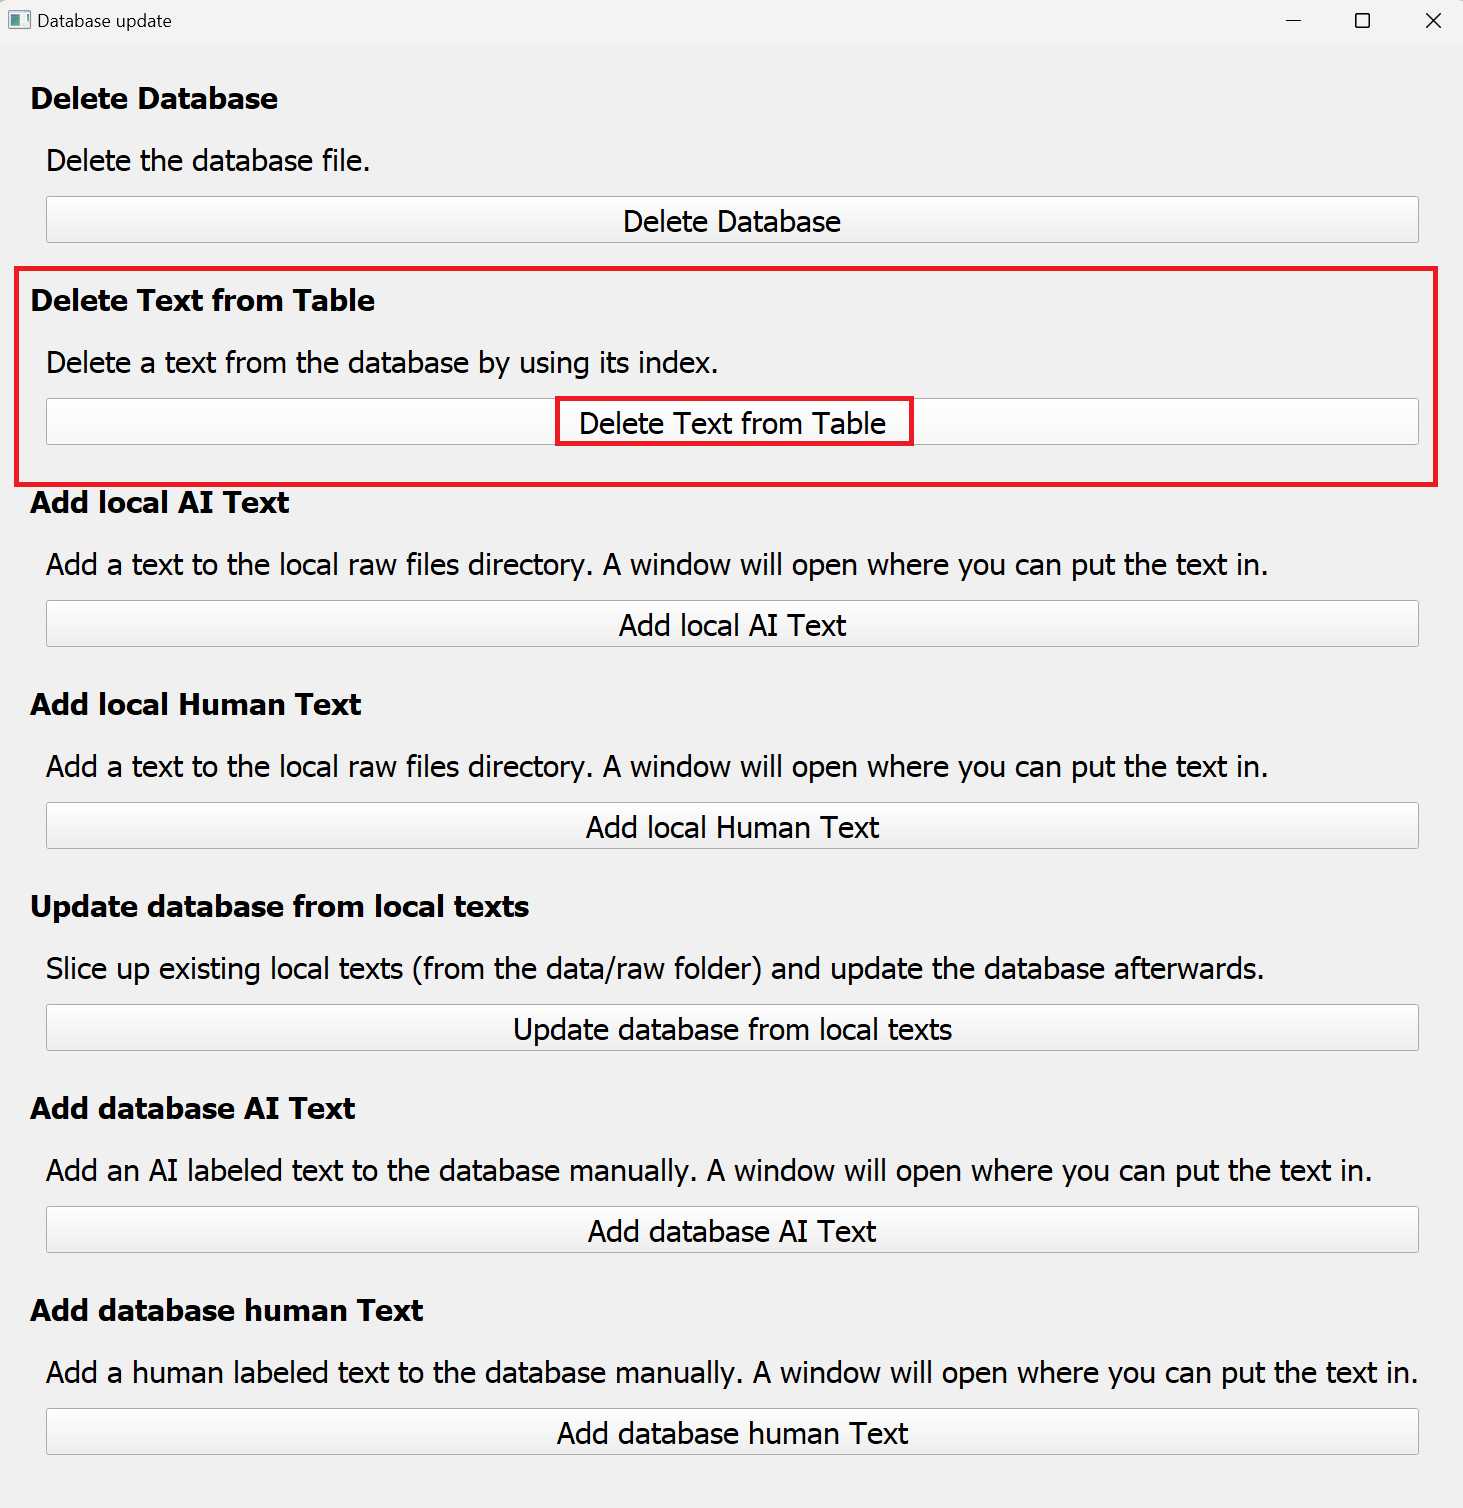
\includegraphics[width=11cm]{Images/Usage/Demo/delete.png}
    \end{center}
    \item On the newly opened deletion window, select the text to delete from the preview list by ticking the corresponding box and then click on the \texttt{Delete Selected} button to confirm. Deletion will output the result under the preview panel.
    \begin{center}
        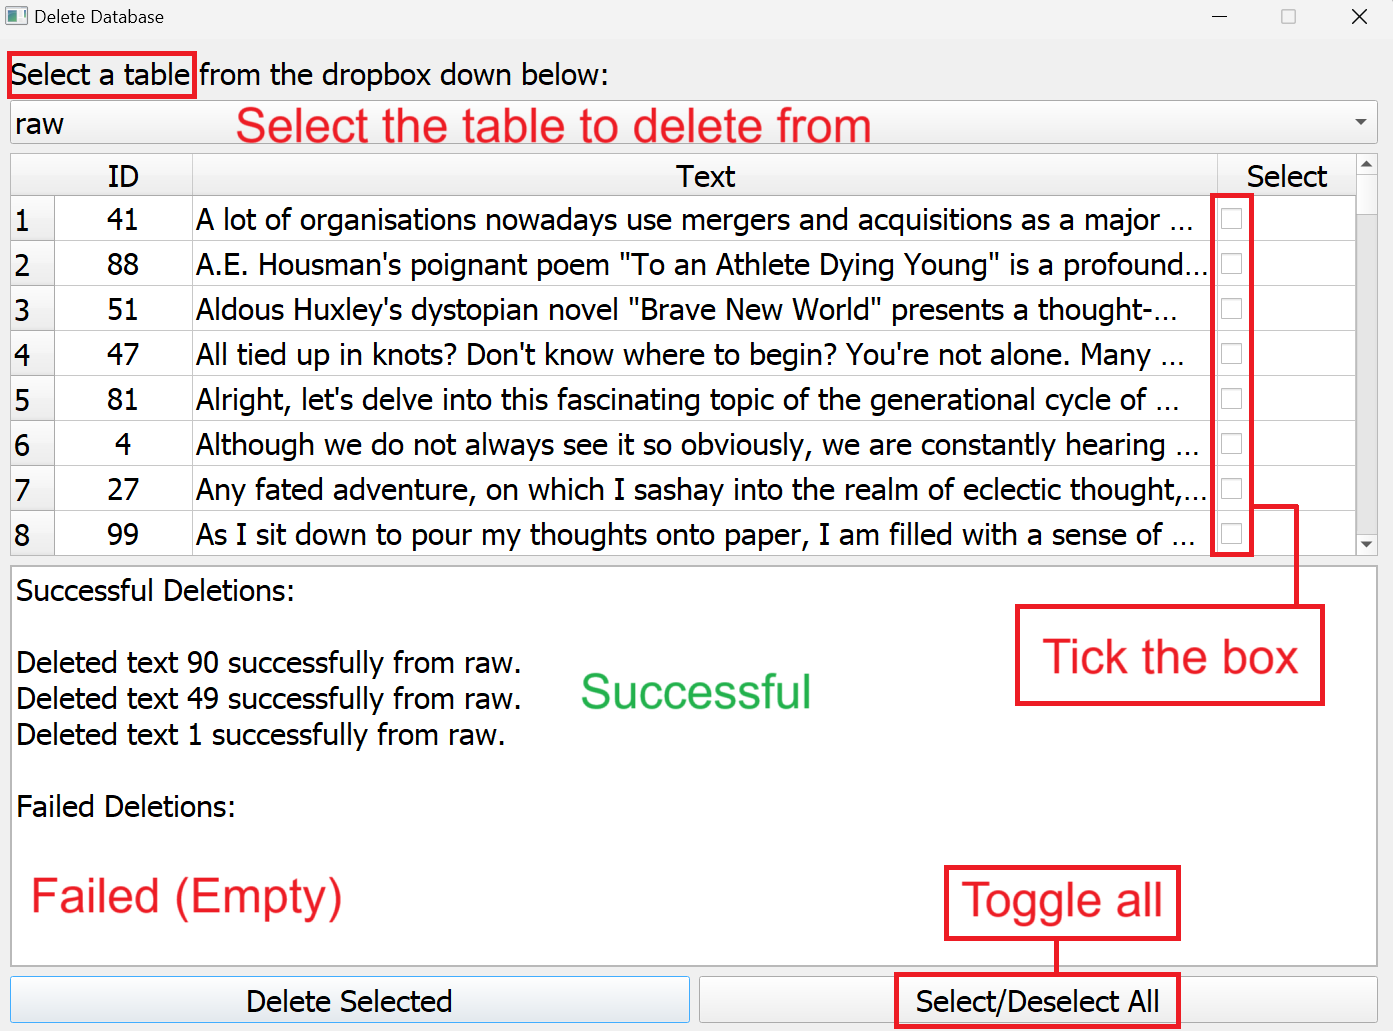
\includegraphics[width=16.5cm]{Images/Usage/Demo/Deletion.png}
    \end{center}
\end{enumerate}
\clearpage
\subsubsection{How to use the local application to train, test and validate models with a new configuration?}
\begin{enumerate}
    \item Open the \hyperref[subsubsec:Web application]{web-based} version of the application or launch the \hyperref[subsubsec:Local application]{local} application using the appropriate method from the \hyperref[subsec:First steps]{installation} steps.
    \item If you have the desired configuration, you can skip to step 4, else navigate to the \hyperref[subsubsec:configuration]{Configuration} sub-window.
    \begin{center}
        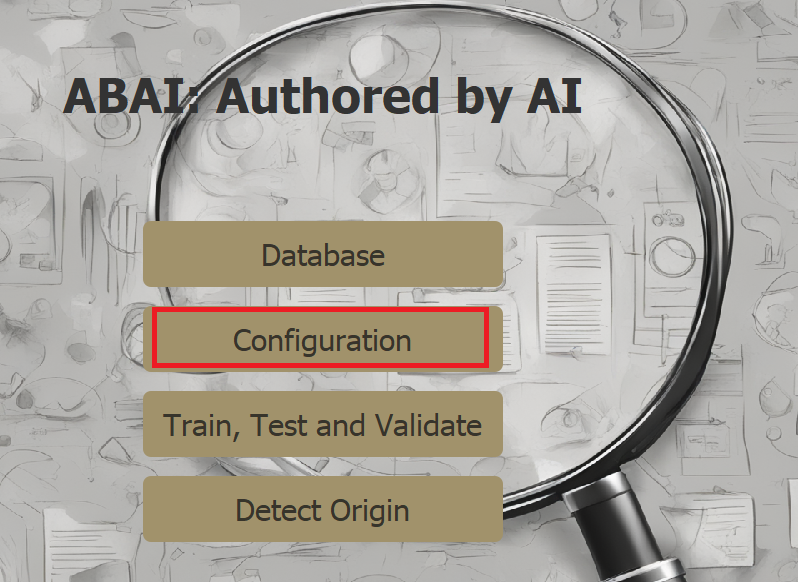
\includegraphics[width=10.5cm]{Images/Usage/Demo/config.png}
    \end{center}
    \item On the Configuration sub-window select the options (brief explanation \hyperref[subsubsec:config-brief-explain]{here}) you want. To illustrate this example, let's say we only want to keep all features extracted before pre-processing.
    \begin{center}
        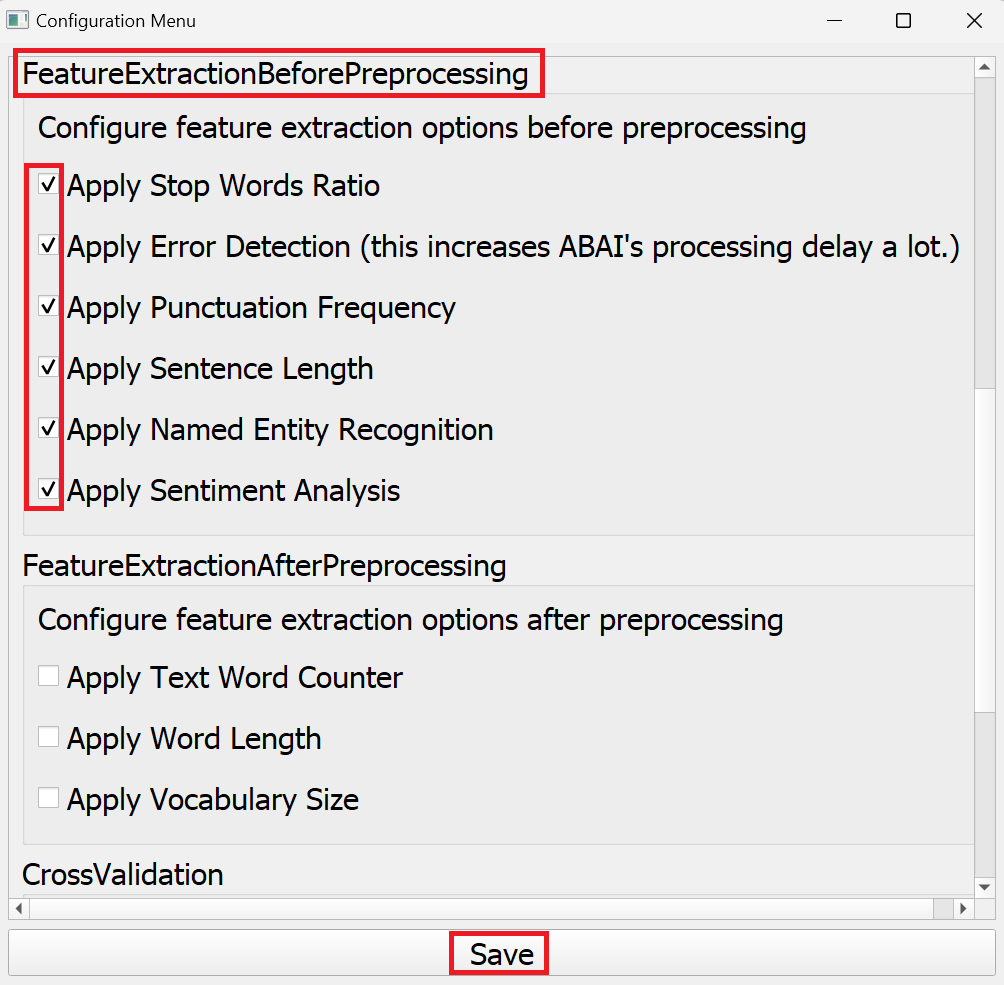
\includegraphics[width=10.5cm]{Images/Usage/Demo/train-config.png}
    \end{center}
    \item Navigate from the main menu to the \hyperref[subsubsec:train-test-validate]{Train, Test and Validate} sub-window.
    \begin{center}
        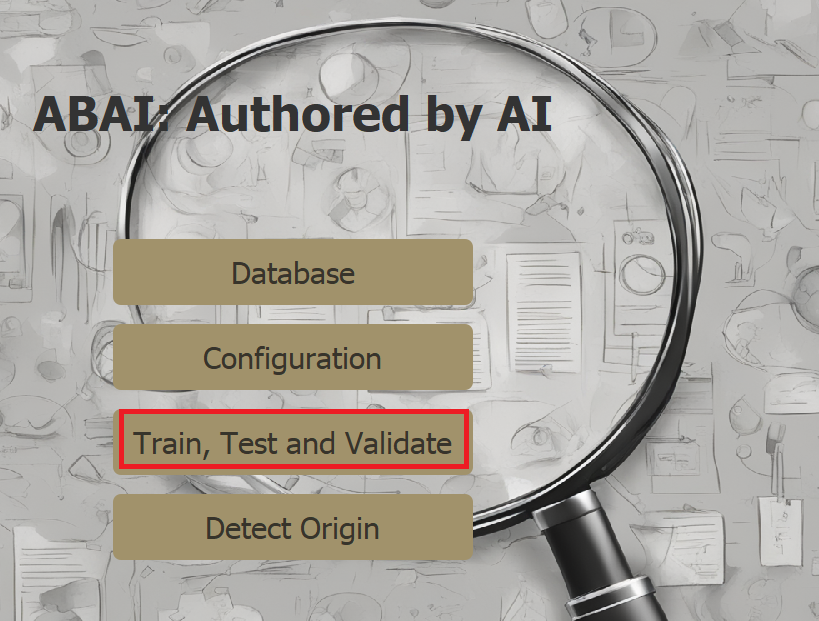
\includegraphics[width=14cm]{Images/Usage/Demo/train-test-validate.png}
    \end{center}
    \item On the Train, Test and Validate sub-window select the action you want to perform. For this how-to, select \texttt{Train, validate and test} from the dropdown list.
    \begin{center}
        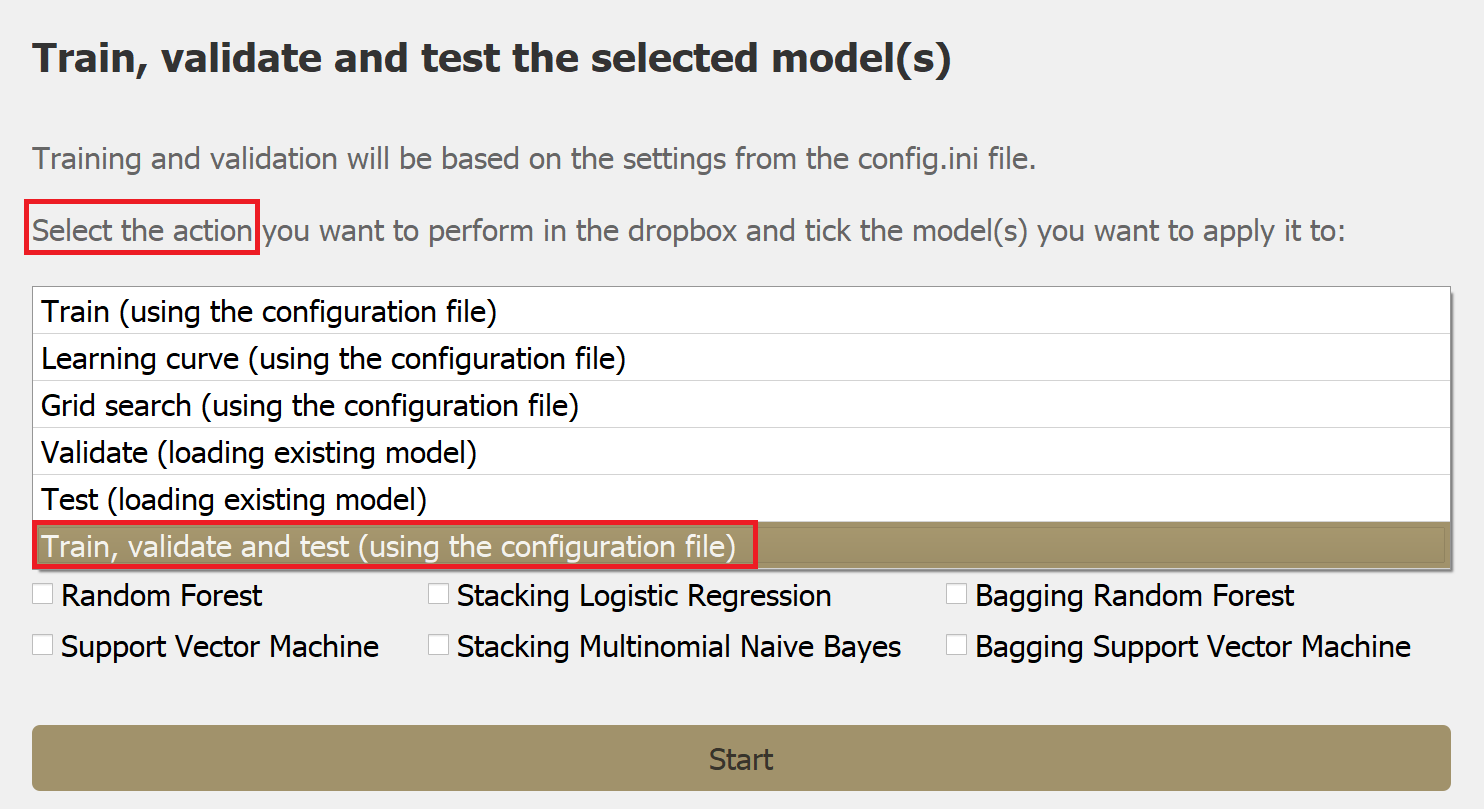
\includegraphics[width=14cm]{Images/Usage/Demo/train-select.png}
    \end{center}
    \clearpage
    \item On the same window, select the model(s) to perform the action on, by ticking the corresponding box and then click on the \texttt{Start} button to confirm. 
    \begin{center}
        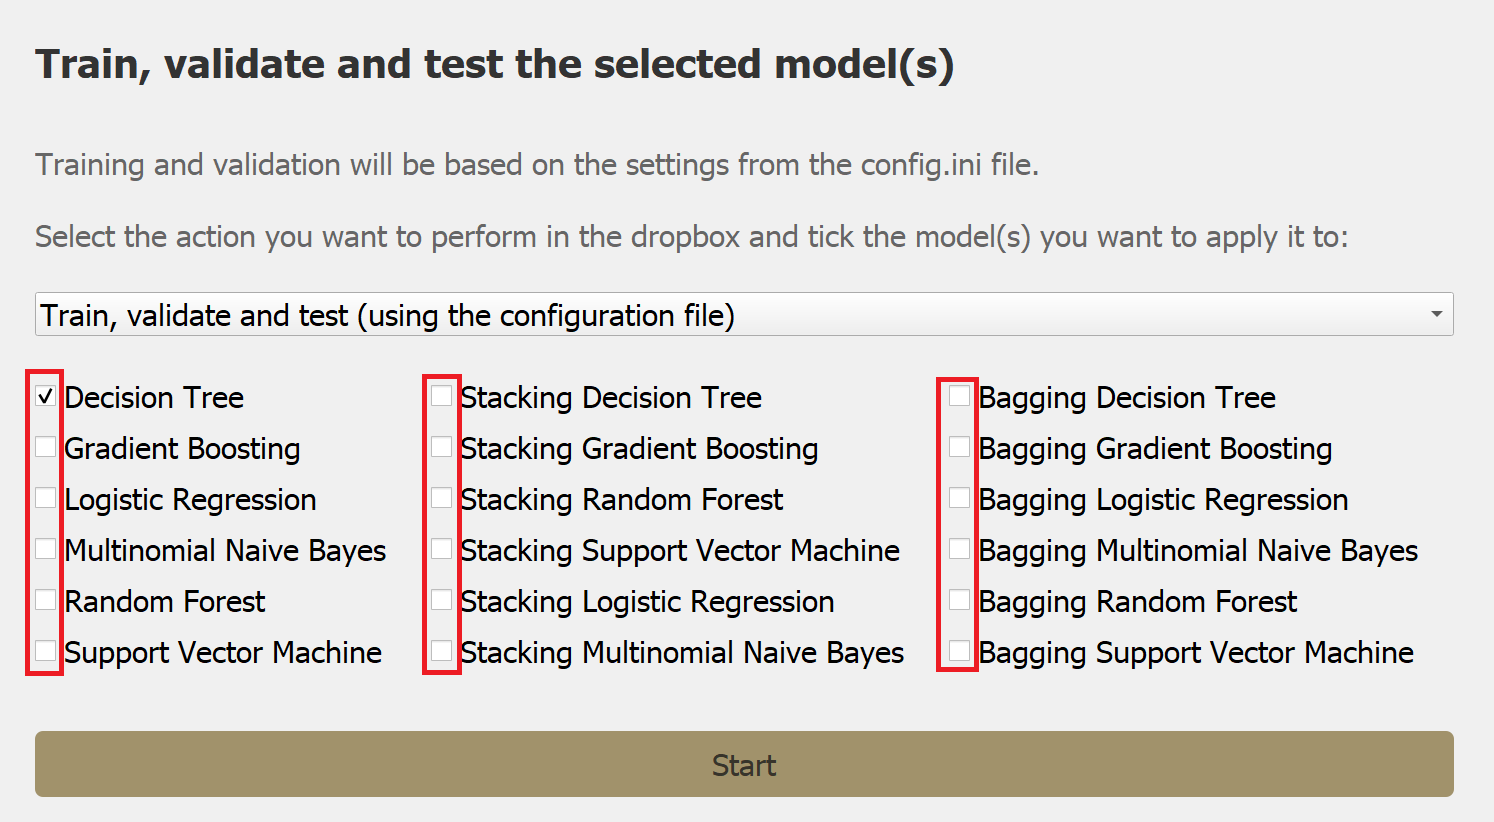
\includegraphics[width=14cm]{Images/Usage/Demo/train-model.png}
    \end{center}
    \item Please wait patiently for the action to finish, the window may look stuck for a while depending on the complexity of the action. When ready, a new window will open to display the results.
    \begin{center}
        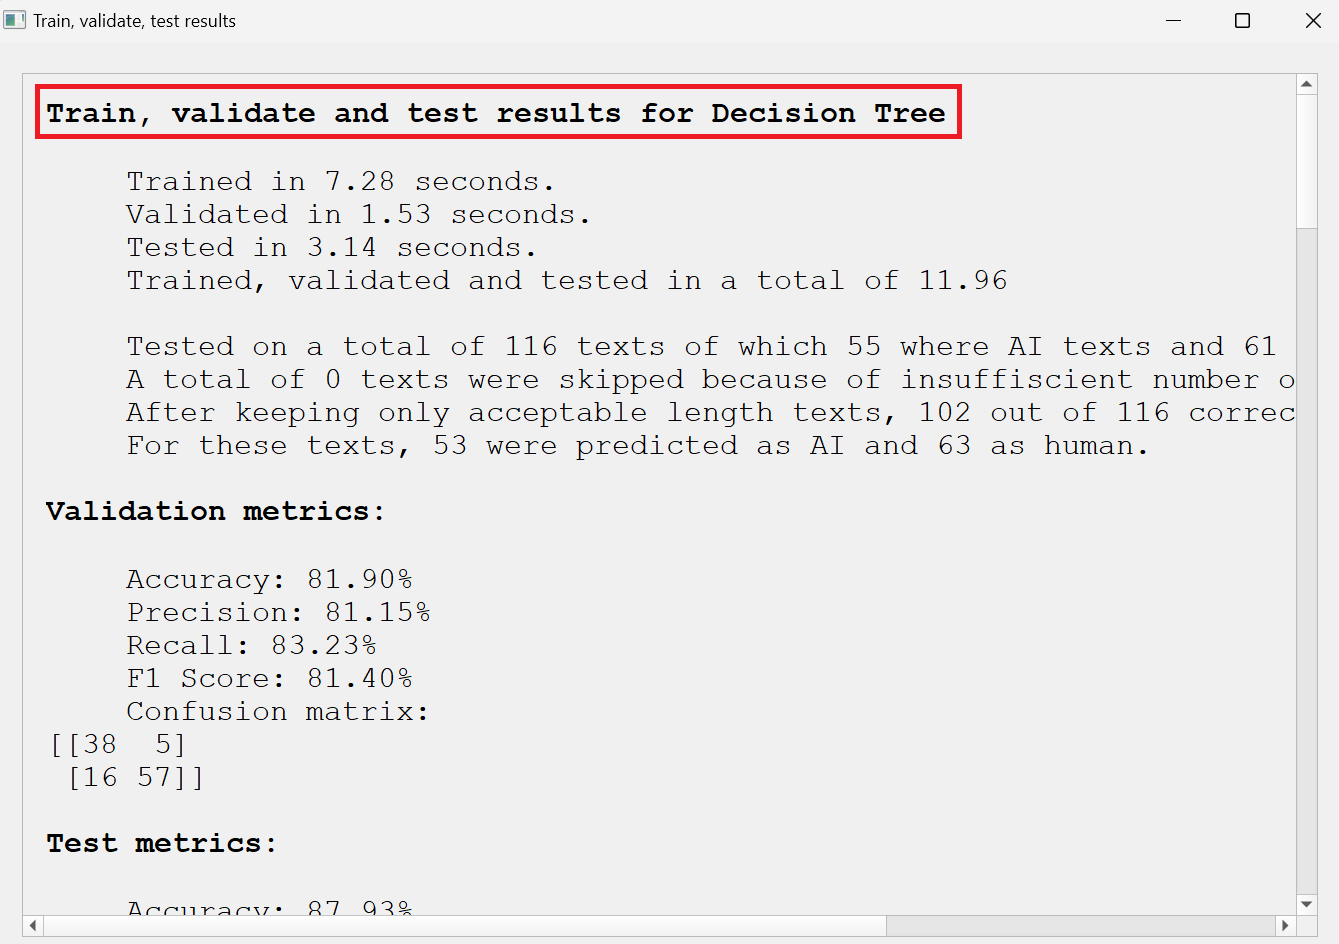
\includegraphics[width=14cm]{Images/Usage/Demo/train-result.png}
    \end{center}
\end{enumerate}
\clearpage
\section{Help}
\subsection{Troubleshooting}
\subsubsection{Pip is not recognized as internal/external command}
\textbf{Error Message:} This error occurs when \texttt{pip} is not in your PATH environment variable. You can try the following instructions to solve this problem:
\begin{enumerate}
    \item If you are running Linux, try using \texttt{pip3} instead of \texttt{pip}.
    \item Add \texttt{pip} to your PATH environment variable by following this \href{https://www.geeksforgeeks.org/how-to-install-  pip-on-windows/}{tutorial}.
    \item Reinstall Python and \texttt{pip}.
\end{enumerate}
\subsubsection{WSL not supported}
The error message indicates that your Windows machine is not able to run WSL. This could be caused by a \textbf{disabled Windows feature} called “Virtual Machine Platform”. WSL depends on it. And in turn, Docker Desktop depends on WSL.

For more information on WSL and \textbf{virtualisation} on windows, please check out the following guides : 

\begin{enumerate}
    \item \href{https://learn.microsoft.com/en-us/windows/wsl/troubleshooting}{Windows Subsystem for Linux}
    \item \href{https://support.microsoft.com/en-us/windows/enable-virtualization-on-windows-11-pcs-c5578302-6e43-4b4b-a449-8ced115f58e1}{Windows 11 Virtualisation}
    \item \href{https://learn.microsoft.com/en-us/virtualization/hyper-v-on-windows/quick-start/enable-hyper-v}{Windows 10 Hyper-V}
\end{enumerate}
\clearpage
\subsection{FAQ}
\subsubsection{I have unintentionally deleted the database, what do I do now?}
You can regenerate the database at all times from the local .TXT files that are shipped with the program or that you have saved yourself. To do this, check out the \hyperref[subsubsec:database]{Database} sub-window.

\subsubsection{Is it possible to perform actions on all models at once?}
Yes, you are always able to select a single or \textbf{multiple} models \textbf{simultaneously} to perform actions on them. This is especially interesting if you decide to change around settings in the configuration file and want to train, validate or test models in \textbf{bulk}. 

\subsubsection{I have used every option from the configuration menu. Is it supposed to be this slow?}
During feature extraction before pre-processing, if error detection is enabled as feature, the computation will be slowed down significantly because of multiple API calls to the \href{https://languagetool.org/http-api/}{LanguageTool API}.

\subsubsection{The Python GUI window is stuck and doesn't respond to input. What can I do ?}
If this happened while performing a complex and resource intensive task and you estimate having waited for long enough, try shrinking the task into smaller and easier sub-tasks to check if it's a performance issue. \\
\newline If the issue persists and you remember how to replicate the issue, you could also \hyperref[sec:contact]{contact} me with the details and I'll look into it. Furthermore, you can open an issue ticket on the \href{https://github.com/UNamurCSFaculty/2324_INFOB318_ABAI2/issues}{GitHub} page of the ABAI project. Every feedback is welcome ! 

\clearpage
\section{About}
\label{sec:About}
\subsection{License}
\label{subsec:License}
\subsubsection{Can I redistribute the application ?}
Yes, you can redistribute the application even under another license, but you must be cautious about how you handle the GPL3-licensed Python module. The GPL3 license requires that any derivative work or modifications made to the GPL3-licensed module must also be licensed under the GPL3 or a compatible license. Therefore, if your modifications are to the GPL3-licensed module itself, those modifications must also be released under the GPL3 license.
\subsubsection{Can I modify the application?}
Yes, you can modify the application, but again, you need to consider the implications of the GPL3 license for the module. If your modifications are limited to the MIT-licensed parts of the application and do not involve modifications to the GPL3-licensed module, then you are free to modify the MIT-licensed portions as you see fit. However, if your modifications extend to the GPL3-licensed module, those modifications must comply with the GPL3 license terms, including the requirement to release the modified code under the GPL3 or a compatible license.
\subsection{Contact}
\label{sec:contact}
If you have any questions or requests, feel free to send me an email at the following address: \href{mailto:Kevin.schweitzer@student.unamur.be}{\nolinkurl{Kevin.schweitzer@student.unamur.be}}

\clearpage
\end{Large}
\end{document}

